% =============================================================================
% InstructorHandouts/CS401/08-io-techniques-instructor-handout.tex
% Instructor Handout 8: I/O Techniques (Interrupts, Polling, Buses, DMA, IOP)
%
% INSTRUCTOR-ONLY. Not published to docs/ (no sync step exists for
% InstructorHandouts/, matching the precedent of Lectures 01-07).
%
% Explanations trace to Slides/CS401/08-io-techniques.tex and
% Notes/CS401/08-io-techniques-notes.tex (the source of truth). All six TikZ
% diagrams are ported verbatim from the Beamer source. Delivery commentary
% (misconceptions, live questions, board sequencing) is instructor judgment and
% is visually marked with the teachingaside environment.
%
% Compile with: cd InstructorHandouts/CS401 &&
%   TEXINPUTS=../../Preambles;$TEXINPUTS xelatex -interaction=nonstopmode 08-io-techniques-instructor-handout.tex
%   (Windows/MiKTeX uses ; not : as the path separator)
% =============================================================================

\documentclass[11pt]{article}
\usepackage[margin=1in]{geometry}
% =============================================================================
% Preambles/header.tex — shared LaTeX/Beamer preamble for this project
%
% Use from a Beamer lecture by prepending:
%     % =============================================================================
% Preambles/header.tex — shared LaTeX/Beamer preamble for this project
%
% Use from a Beamer lecture by prepending:
%     % =============================================================================
% Preambles/header.tex — shared LaTeX/Beamer preamble for this project
%
% Use from a Beamer lecture by prepending:
%     \input{header}
% and compiling with TEXINPUTS=../Preambles:$TEXINPUTS (the /compile-latex
% skill does this automatically).
%
% PALETTE CONTRACT. Color names defined here MUST match the names in
% Quarto/theme-template.scss so Beamer and Quarto renderings use the same
% palette. The scripts/check-palette-sync.sh script enforces this.
%
% To customize: edit the HEX values below AND the matching $variable in
% Quarto/theme-template.scss, then run scripts/check-palette-sync.sh.
%
% TITLE PAGE. A formal, serif (Libertine) title-page template is defined in
% the Beamer-only block below (\setbeamertemplate{title page}) -- title,
% subtitle, a thin gold rule, then \author/\institute/\date. Frametitle and
% body text remain on Beamer's sans-serif default. No SCSS counterpart is
% needed for this (font/layout only, no new colors).
% =============================================================================

% -----------------------------------------------------------------------------
% Engine detection + encoding
%
% Our /compile-latex skill uses XeLaTeX, where inputenc is unnecessary and
% can produce encoding warnings. Only load inputenc under pdfTeX.
% -----------------------------------------------------------------------------
\usepackage{iftex}
\ifPDFTeX
  \usepackage[utf8]{inputenc}
\fi

\usepackage{amsmath, amssymb, amsthm}
\usepackage{booktabs}
\usepackage{graphicx}

% -----------------------------------------------------------------------------
% Serif face for the title page (formal/academic look). Linux Libertine is
% XeLaTeX- and pdfTeX-safe and redefines \rmdefault, so \rmfamily picks it up
% everywhere \rmfamily is used explicitly. Body text and frametitles stay on
% Beamer's own sans-serif default (unaffected) -- only the title-page
% \setbeamerfont{...} overrides below opt in to \rmfamily.
% -----------------------------------------------------------------------------
\usepackage{libertine}

% -----------------------------------------------------------------------------
% PALETTE — mirrors Quarto/theme-template.scss variable names.
% Load xcolor and define colors BEFORE anything that references them
% (notably hyperref, hypersetup, and the Beamer color assignments).
% -----------------------------------------------------------------------------
\usepackage{xcolor}

\definecolor{primary-blue}{HTML}{012169}      % headings, accents
\definecolor{primary-gold}{HTML}{B9975B}      % emphasis, borders
\definecolor{highlight-yellow}{HTML}{F2A900}  % markers, alerts
\definecolor{light-bg}{HTML}{E8EDF5}          % title / section backgrounds
\definecolor{jet}{HTML}{1A1A1A}               % body text

% Semantic colors (used in diagrams and annotations)
\definecolor{positive}{HTML}{15803D}          % good / observed / identified
\definecolor{negative}{HTML}{B91C1C}          % bad / problematic / bias
\definecolor{neutral}{HTML}{525252}           % reference / context

% Highlight accents (match .hi-* classes in the SCSS)
\definecolor{hi-slate}{HTML}{314F4F}
\definecolor{hi-green}{HTML}{2E8B57}
\definecolor{hi-red}{HTML}{C41E3A}

% Semantic aliases so skill templates and snippets can write
% \textcolor{accent}{...} without hard-coding "primary-blue".
\colorlet{accent}{primary-blue}
\colorlet{accent2}{primary-gold}

% -----------------------------------------------------------------------------
% Hyperref — loaded AFTER xcolor + palette so link colors resolve.
% -----------------------------------------------------------------------------
\usepackage{hyperref}
\hypersetup{colorlinks=true, linkcolor=primary-blue, urlcolor=primary-blue,
            citecolor=primary-blue, pdfborder={0 0 0}}

% -----------------------------------------------------------------------------
% Course code — set once per deck (after \input{header}, before \begin{document})
% via \coursecode{CS401}. Shown in the footer on every slide so a deck's course
% is identifiable without opening the title page. Empty by default.
% -----------------------------------------------------------------------------
\makeatletter
\newcommand{\coursecode}[1]{\gdef\@coursecodetext{#1}}
\gdef\@coursecodetext{}
\makeatother

% -----------------------------------------------------------------------------
% Beamer theme assignments (only apply under Beamer).
%
% We detect Beamer via \@ifclassloaded{beamer}, which is the documented,
% non-internal way. This must be wrapped in \makeatletter/\makeatother
% because \@ifclassloaded contains an @-catcode character.
% -----------------------------------------------------------------------------
\makeatletter
\@ifclassloaded{beamer}{%
  \usefonttheme{professionalfonts}
  \setbeamercolor{structure}{fg=primary-blue}
  \setbeamercolor{frametitle}{fg=primary-blue}
  \setbeamercolor{title}{fg=primary-blue}
  \setbeamercolor{subtitle}{fg=primary-gold}
  \setbeamercolor{author}{fg=primary-blue}
  \setbeamercolor{institute}{fg=neutral}
  \setbeamercolor{date}{fg=primary-gold}
  \setbeamercolor{itemize item}{fg=primary-blue}
  \setbeamercolor{itemize subitem}{fg=primary-gold}
  \setbeamercolor{alerted text}{fg=primary-gold}
  \setbeamercolor{block title}{fg=white, bg=primary-blue}
  \setbeamercolor{block body}{bg=light-bg}
  % Semantic block variants: block=definition/concept (blue), exampleblock=
  % worked example (green/positive), alertblock=key takeaway or caution (gold).
  % Keep to <=2 colored boxes per slide across ALL three variants (INV-7).
  \setbeamercolor{block title example}{fg=white, bg=positive}
  \setbeamercolor{block body example}{bg=light-bg}
  \setbeamercolor{block title alerted}{fg=white, bg=primary-gold}
  \setbeamercolor{block body alerted}{bg=light-bg}

  % ---------------------------------------------------------------------------
  % Formal title page: serif (Libertine, via \rmfamily) for title-page
  % elements only. Body text, itemize, and frametitle are intentionally left
  % on Beamer's sans-serif default -- \usebeamerfont{title} is also what
  % \transitionslide (below) uses for its big centered text, so section
  % transitions pick up the same serif treatment for free.
  % ---------------------------------------------------------------------------
  \setbeamerfont{title}{family=\rmfamily, series=\bfseries, size=\Large}
  \setbeamerfont{subtitle}{family=\rmfamily, shape=\itshape, size=\normalsize}
  \setbeamerfont{author}{family=\rmfamily, size=\normalsize}
  \setbeamerfont{institute}{family=\rmfamily, size=\scriptsize}
  \setbeamerfont{date}{family=\rmfamily, size=\scriptsize}

  \setbeamertemplate{title page}{
    \vfill
    \begin{center}
      {\usebeamerfont{title}\usebeamercolor[fg]{title}\inserttitle\par}
      \vspace{0.15cm}
      {\usebeamerfont{subtitle}\usebeamercolor[fg]{subtitle}\insertsubtitle\par}
      \vspace{0.45cm}
      {\color{primary-gold}\rule{0.42\textwidth}{0.6pt}\par}
      \vspace{0.45cm}
      {\usebeamerfont{author}\usebeamercolor[fg]{author}\insertauthor\par}
      \vspace{0.35cm}
      {\usebeamerfont{institute}\usebeamercolor[fg]{institute}\insertinstitute\par}
      \vspace{0.35cm}
      {\usebeamerfont{date}\usebeamercolor[fg]{date}\insertdate\par}
    \end{center}
    \vfill
  }

  % Minimal footer: course code (left) + page X / N (right), no navigation clutter
  \setbeamertemplate{navigation symbols}{}
  \setbeamertemplate{footline}{%
    \color{neutral}\footnotesize\hspace{0.7em}\@coursecodetext\hfill
    \insertframenumber/\inserttotalframenumber\hspace{0.7em}\vspace{0.3em}}
}{}
\makeatother

% -----------------------------------------------------------------------------
% TikZ setup — libraries the snippet gallery uses
% -----------------------------------------------------------------------------
\usepackage{tikz}
\usetikzlibrary{arrows.meta, positioning, calc, decorations.pathreplacing,
                fit, shapes.geometric, backgrounds}

% Shared TikZ styles — snippets and hand-written diagrams can pick these up
% via `\begin{tikzpicture}[every node/.style={...}]` or by naming specific
% styles (e.g., `\node[dag-node] (X) at (0,0) {X};`).
\tikzset{
  % Node styles for causal DAGs and similar
  dag-node/.style = {
    draw=primary-blue, fill=light-bg, rounded corners=2pt,
    minimum width=1.2cm, minimum height=0.9cm, align=center, font=\small
  },
  decision-node/.style = {
    draw=primary-gold, fill=white, diamond, aspect=1.8,
    minimum width=1.8cm, minimum height=1.2cm, align=center, font=\small,
    inner sep=1pt
  },
  % Edge styles — observed vs counterfactual
  observed-edge/.style = {-{Latex[length=2.5mm]}, thick, draw=jet},
  counterfactual-edge/.style = {-{Latex[length=2.5mm]}, thick, draw=neutral, dashed},
  confound-edge/.style = {-{Latex[length=2.5mm]}, thick, draw=negative, dashed},
  % Data-point styles for plots
  observed-dot/.style = {fill=primary-blue, draw=primary-blue, circle, inner sep=1.2pt},
  counterfactual-dot/.style = {fill=white, draw=neutral, circle, inner sep=1.2pt}
}

% -----------------------------------------------------------------------------
% Convenience macros
% -----------------------------------------------------------------------------
\newcommand{\muted}[1]{\textcolor{neutral}{#1}}
\newcommand{\key}[1]{\textcolor{primary-gold}{\textbf{#1}}}
\newcommand{\good}[1]{\textcolor{positive}{#1}}
\newcommand{\bad}[1]{\textcolor{negative}{#1}}

% Standout frame macro: full-bleed dark background for section transitions.
% Beamer-only (uses \begin{frame}/\setbeamercolor/\usebeamerfont) -- do not
% call from an article-class file (e.g. Notes/<CODE>/*-notes.tex). \muted,
% \key, \good, \bad, and \coursecode above are plain xcolor/gdef and are
% safe to use from either class; verified when Notes/article-class support
% was added.
% Expand: \transitionslide{Your transition title}
\newcommand{\transitionslide}[1]{%
  \begingroup
  \setbeamercolor{background canvas}{bg=primary-blue}
  \begin{frame}[plain]
    \centering
    \vfill
    {\usebeamerfont{title}\color{white}\Large #1\par}
    \vfill
  \end{frame}
  \endgroup
}

% and compiling with TEXINPUTS=../Preambles:$TEXINPUTS (the /compile-latex
% skill does this automatically).
%
% PALETTE CONTRACT. Color names defined here MUST match the names in
% Quarto/theme-template.scss so Beamer and Quarto renderings use the same
% palette. The scripts/check-palette-sync.sh script enforces this.
%
% To customize: edit the HEX values below AND the matching $variable in
% Quarto/theme-template.scss, then run scripts/check-palette-sync.sh.
%
% TITLE PAGE. A formal, serif (Libertine) title-page template is defined in
% the Beamer-only block below (\setbeamertemplate{title page}) -- title,
% subtitle, a thin gold rule, then \author/\institute/\date. Frametitle and
% body text remain on Beamer's sans-serif default. No SCSS counterpart is
% needed for this (font/layout only, no new colors).
% =============================================================================

% -----------------------------------------------------------------------------
% Engine detection + encoding
%
% Our /compile-latex skill uses XeLaTeX, where inputenc is unnecessary and
% can produce encoding warnings. Only load inputenc under pdfTeX.
% -----------------------------------------------------------------------------
\usepackage{iftex}
\ifPDFTeX
  \usepackage[utf8]{inputenc}
\fi

\usepackage{amsmath, amssymb, amsthm}
\usepackage{booktabs}
\usepackage{graphicx}

% -----------------------------------------------------------------------------
% Serif face for the title page (formal/academic look). Linux Libertine is
% XeLaTeX- and pdfTeX-safe and redefines \rmdefault, so \rmfamily picks it up
% everywhere \rmfamily is used explicitly. Body text and frametitles stay on
% Beamer's own sans-serif default (unaffected) -- only the title-page
% \setbeamerfont{...} overrides below opt in to \rmfamily.
% -----------------------------------------------------------------------------
\usepackage{libertine}

% -----------------------------------------------------------------------------
% PALETTE — mirrors Quarto/theme-template.scss variable names.
% Load xcolor and define colors BEFORE anything that references them
% (notably hyperref, hypersetup, and the Beamer color assignments).
% -----------------------------------------------------------------------------
\usepackage{xcolor}

\definecolor{primary-blue}{HTML}{012169}      % headings, accents
\definecolor{primary-gold}{HTML}{B9975B}      % emphasis, borders
\definecolor{highlight-yellow}{HTML}{F2A900}  % markers, alerts
\definecolor{light-bg}{HTML}{E8EDF5}          % title / section backgrounds
\definecolor{jet}{HTML}{1A1A1A}               % body text

% Semantic colors (used in diagrams and annotations)
\definecolor{positive}{HTML}{15803D}          % good / observed / identified
\definecolor{negative}{HTML}{B91C1C}          % bad / problematic / bias
\definecolor{neutral}{HTML}{525252}           % reference / context

% Highlight accents (match .hi-* classes in the SCSS)
\definecolor{hi-slate}{HTML}{314F4F}
\definecolor{hi-green}{HTML}{2E8B57}
\definecolor{hi-red}{HTML}{C41E3A}

% Semantic aliases so skill templates and snippets can write
% \textcolor{accent}{...} without hard-coding "primary-blue".
\colorlet{accent}{primary-blue}
\colorlet{accent2}{primary-gold}

% -----------------------------------------------------------------------------
% Hyperref — loaded AFTER xcolor + palette so link colors resolve.
% -----------------------------------------------------------------------------
\usepackage{hyperref}
\hypersetup{colorlinks=true, linkcolor=primary-blue, urlcolor=primary-blue,
            citecolor=primary-blue, pdfborder={0 0 0}}

% -----------------------------------------------------------------------------
% Course code — set once per deck (after % =============================================================================
% Preambles/header.tex — shared LaTeX/Beamer preamble for this project
%
% Use from a Beamer lecture by prepending:
%     \input{header}
% and compiling with TEXINPUTS=../Preambles:$TEXINPUTS (the /compile-latex
% skill does this automatically).
%
% PALETTE CONTRACT. Color names defined here MUST match the names in
% Quarto/theme-template.scss so Beamer and Quarto renderings use the same
% palette. The scripts/check-palette-sync.sh script enforces this.
%
% To customize: edit the HEX values below AND the matching $variable in
% Quarto/theme-template.scss, then run scripts/check-palette-sync.sh.
%
% TITLE PAGE. A formal, serif (Libertine) title-page template is defined in
% the Beamer-only block below (\setbeamertemplate{title page}) -- title,
% subtitle, a thin gold rule, then \author/\institute/\date. Frametitle and
% body text remain on Beamer's sans-serif default. No SCSS counterpart is
% needed for this (font/layout only, no new colors).
% =============================================================================

% -----------------------------------------------------------------------------
% Engine detection + encoding
%
% Our /compile-latex skill uses XeLaTeX, where inputenc is unnecessary and
% can produce encoding warnings. Only load inputenc under pdfTeX.
% -----------------------------------------------------------------------------
\usepackage{iftex}
\ifPDFTeX
  \usepackage[utf8]{inputenc}
\fi

\usepackage{amsmath, amssymb, amsthm}
\usepackage{booktabs}
\usepackage{graphicx}

% -----------------------------------------------------------------------------
% Serif face for the title page (formal/academic look). Linux Libertine is
% XeLaTeX- and pdfTeX-safe and redefines \rmdefault, so \rmfamily picks it up
% everywhere \rmfamily is used explicitly. Body text and frametitles stay on
% Beamer's own sans-serif default (unaffected) -- only the title-page
% \setbeamerfont{...} overrides below opt in to \rmfamily.
% -----------------------------------------------------------------------------
\usepackage{libertine}

% -----------------------------------------------------------------------------
% PALETTE — mirrors Quarto/theme-template.scss variable names.
% Load xcolor and define colors BEFORE anything that references them
% (notably hyperref, hypersetup, and the Beamer color assignments).
% -----------------------------------------------------------------------------
\usepackage{xcolor}

\definecolor{primary-blue}{HTML}{012169}      % headings, accents
\definecolor{primary-gold}{HTML}{B9975B}      % emphasis, borders
\definecolor{highlight-yellow}{HTML}{F2A900}  % markers, alerts
\definecolor{light-bg}{HTML}{E8EDF5}          % title / section backgrounds
\definecolor{jet}{HTML}{1A1A1A}               % body text

% Semantic colors (used in diagrams and annotations)
\definecolor{positive}{HTML}{15803D}          % good / observed / identified
\definecolor{negative}{HTML}{B91C1C}          % bad / problematic / bias
\definecolor{neutral}{HTML}{525252}           % reference / context

% Highlight accents (match .hi-* classes in the SCSS)
\definecolor{hi-slate}{HTML}{314F4F}
\definecolor{hi-green}{HTML}{2E8B57}
\definecolor{hi-red}{HTML}{C41E3A}

% Semantic aliases so skill templates and snippets can write
% \textcolor{accent}{...} without hard-coding "primary-blue".
\colorlet{accent}{primary-blue}
\colorlet{accent2}{primary-gold}

% -----------------------------------------------------------------------------
% Hyperref — loaded AFTER xcolor + palette so link colors resolve.
% -----------------------------------------------------------------------------
\usepackage{hyperref}
\hypersetup{colorlinks=true, linkcolor=primary-blue, urlcolor=primary-blue,
            citecolor=primary-blue, pdfborder={0 0 0}}

% -----------------------------------------------------------------------------
% Course code — set once per deck (after \input{header}, before \begin{document})
% via \coursecode{CS401}. Shown in the footer on every slide so a deck's course
% is identifiable without opening the title page. Empty by default.
% -----------------------------------------------------------------------------
\makeatletter
\newcommand{\coursecode}[1]{\gdef\@coursecodetext{#1}}
\gdef\@coursecodetext{}
\makeatother

% -----------------------------------------------------------------------------
% Beamer theme assignments (only apply under Beamer).
%
% We detect Beamer via \@ifclassloaded{beamer}, which is the documented,
% non-internal way. This must be wrapped in \makeatletter/\makeatother
% because \@ifclassloaded contains an @-catcode character.
% -----------------------------------------------------------------------------
\makeatletter
\@ifclassloaded{beamer}{%
  \usefonttheme{professionalfonts}
  \setbeamercolor{structure}{fg=primary-blue}
  \setbeamercolor{frametitle}{fg=primary-blue}
  \setbeamercolor{title}{fg=primary-blue}
  \setbeamercolor{subtitle}{fg=primary-gold}
  \setbeamercolor{author}{fg=primary-blue}
  \setbeamercolor{institute}{fg=neutral}
  \setbeamercolor{date}{fg=primary-gold}
  \setbeamercolor{itemize item}{fg=primary-blue}
  \setbeamercolor{itemize subitem}{fg=primary-gold}
  \setbeamercolor{alerted text}{fg=primary-gold}
  \setbeamercolor{block title}{fg=white, bg=primary-blue}
  \setbeamercolor{block body}{bg=light-bg}
  % Semantic block variants: block=definition/concept (blue), exampleblock=
  % worked example (green/positive), alertblock=key takeaway or caution (gold).
  % Keep to <=2 colored boxes per slide across ALL three variants (INV-7).
  \setbeamercolor{block title example}{fg=white, bg=positive}
  \setbeamercolor{block body example}{bg=light-bg}
  \setbeamercolor{block title alerted}{fg=white, bg=primary-gold}
  \setbeamercolor{block body alerted}{bg=light-bg}

  % ---------------------------------------------------------------------------
  % Formal title page: serif (Libertine, via \rmfamily) for title-page
  % elements only. Body text, itemize, and frametitle are intentionally left
  % on Beamer's sans-serif default -- \usebeamerfont{title} is also what
  % \transitionslide (below) uses for its big centered text, so section
  % transitions pick up the same serif treatment for free.
  % ---------------------------------------------------------------------------
  \setbeamerfont{title}{family=\rmfamily, series=\bfseries, size=\Large}
  \setbeamerfont{subtitle}{family=\rmfamily, shape=\itshape, size=\normalsize}
  \setbeamerfont{author}{family=\rmfamily, size=\normalsize}
  \setbeamerfont{institute}{family=\rmfamily, size=\scriptsize}
  \setbeamerfont{date}{family=\rmfamily, size=\scriptsize}

  \setbeamertemplate{title page}{
    \vfill
    \begin{center}
      {\usebeamerfont{title}\usebeamercolor[fg]{title}\inserttitle\par}
      \vspace{0.15cm}
      {\usebeamerfont{subtitle}\usebeamercolor[fg]{subtitle}\insertsubtitle\par}
      \vspace{0.45cm}
      {\color{primary-gold}\rule{0.42\textwidth}{0.6pt}\par}
      \vspace{0.45cm}
      {\usebeamerfont{author}\usebeamercolor[fg]{author}\insertauthor\par}
      \vspace{0.35cm}
      {\usebeamerfont{institute}\usebeamercolor[fg]{institute}\insertinstitute\par}
      \vspace{0.35cm}
      {\usebeamerfont{date}\usebeamercolor[fg]{date}\insertdate\par}
    \end{center}
    \vfill
  }

  % Minimal footer: course code (left) + page X / N (right), no navigation clutter
  \setbeamertemplate{navigation symbols}{}
  \setbeamertemplate{footline}{%
    \color{neutral}\footnotesize\hspace{0.7em}\@coursecodetext\hfill
    \insertframenumber/\inserttotalframenumber\hspace{0.7em}\vspace{0.3em}}
}{}
\makeatother

% -----------------------------------------------------------------------------
% TikZ setup — libraries the snippet gallery uses
% -----------------------------------------------------------------------------
\usepackage{tikz}
\usetikzlibrary{arrows.meta, positioning, calc, decorations.pathreplacing,
                fit, shapes.geometric, backgrounds}

% Shared TikZ styles — snippets and hand-written diagrams can pick these up
% via `\begin{tikzpicture}[every node/.style={...}]` or by naming specific
% styles (e.g., `\node[dag-node] (X) at (0,0) {X};`).
\tikzset{
  % Node styles for causal DAGs and similar
  dag-node/.style = {
    draw=primary-blue, fill=light-bg, rounded corners=2pt,
    minimum width=1.2cm, minimum height=0.9cm, align=center, font=\small
  },
  decision-node/.style = {
    draw=primary-gold, fill=white, diamond, aspect=1.8,
    minimum width=1.8cm, minimum height=1.2cm, align=center, font=\small,
    inner sep=1pt
  },
  % Edge styles — observed vs counterfactual
  observed-edge/.style = {-{Latex[length=2.5mm]}, thick, draw=jet},
  counterfactual-edge/.style = {-{Latex[length=2.5mm]}, thick, draw=neutral, dashed},
  confound-edge/.style = {-{Latex[length=2.5mm]}, thick, draw=negative, dashed},
  % Data-point styles for plots
  observed-dot/.style = {fill=primary-blue, draw=primary-blue, circle, inner sep=1.2pt},
  counterfactual-dot/.style = {fill=white, draw=neutral, circle, inner sep=1.2pt}
}

% -----------------------------------------------------------------------------
% Convenience macros
% -----------------------------------------------------------------------------
\newcommand{\muted}[1]{\textcolor{neutral}{#1}}
\newcommand{\key}[1]{\textcolor{primary-gold}{\textbf{#1}}}
\newcommand{\good}[1]{\textcolor{positive}{#1}}
\newcommand{\bad}[1]{\textcolor{negative}{#1}}

% Standout frame macro: full-bleed dark background for section transitions.
% Beamer-only (uses \begin{frame}/\setbeamercolor/\usebeamerfont) -- do not
% call from an article-class file (e.g. Notes/<CODE>/*-notes.tex). \muted,
% \key, \good, \bad, and \coursecode above are plain xcolor/gdef and are
% safe to use from either class; verified when Notes/article-class support
% was added.
% Expand: \transitionslide{Your transition title}
\newcommand{\transitionslide}[1]{%
  \begingroup
  \setbeamercolor{background canvas}{bg=primary-blue}
  \begin{frame}[plain]
    \centering
    \vfill
    {\usebeamerfont{title}\color{white}\Large #1\par}
    \vfill
  \end{frame}
  \endgroup
}
, before \begin{document})
% via \coursecode{CS401}. Shown in the footer on every slide so a deck's course
% is identifiable without opening the title page. Empty by default.
% -----------------------------------------------------------------------------
\makeatletter
\newcommand{\coursecode}[1]{\gdef\@coursecodetext{#1}}
\gdef\@coursecodetext{}
\makeatother

% -----------------------------------------------------------------------------
% Beamer theme assignments (only apply under Beamer).
%
% We detect Beamer via \@ifclassloaded{beamer}, which is the documented,
% non-internal way. This must be wrapped in \makeatletter/\makeatother
% because \@ifclassloaded contains an @-catcode character.
% -----------------------------------------------------------------------------
\makeatletter
\@ifclassloaded{beamer}{%
  \usefonttheme{professionalfonts}
  \setbeamercolor{structure}{fg=primary-blue}
  \setbeamercolor{frametitle}{fg=primary-blue}
  \setbeamercolor{title}{fg=primary-blue}
  \setbeamercolor{subtitle}{fg=primary-gold}
  \setbeamercolor{author}{fg=primary-blue}
  \setbeamercolor{institute}{fg=neutral}
  \setbeamercolor{date}{fg=primary-gold}
  \setbeamercolor{itemize item}{fg=primary-blue}
  \setbeamercolor{itemize subitem}{fg=primary-gold}
  \setbeamercolor{alerted text}{fg=primary-gold}
  \setbeamercolor{block title}{fg=white, bg=primary-blue}
  \setbeamercolor{block body}{bg=light-bg}
  % Semantic block variants: block=definition/concept (blue), exampleblock=
  % worked example (green/positive), alertblock=key takeaway or caution (gold).
  % Keep to <=2 colored boxes per slide across ALL three variants (INV-7).
  \setbeamercolor{block title example}{fg=white, bg=positive}
  \setbeamercolor{block body example}{bg=light-bg}
  \setbeamercolor{block title alerted}{fg=white, bg=primary-gold}
  \setbeamercolor{block body alerted}{bg=light-bg}

  % ---------------------------------------------------------------------------
  % Formal title page: serif (Libertine, via \rmfamily) for title-page
  % elements only. Body text, itemize, and frametitle are intentionally left
  % on Beamer's sans-serif default -- \usebeamerfont{title} is also what
  % \transitionslide (below) uses for its big centered text, so section
  % transitions pick up the same serif treatment for free.
  % ---------------------------------------------------------------------------
  \setbeamerfont{title}{family=\rmfamily, series=\bfseries, size=\Large}
  \setbeamerfont{subtitle}{family=\rmfamily, shape=\itshape, size=\normalsize}
  \setbeamerfont{author}{family=\rmfamily, size=\normalsize}
  \setbeamerfont{institute}{family=\rmfamily, size=\scriptsize}
  \setbeamerfont{date}{family=\rmfamily, size=\scriptsize}

  \setbeamertemplate{title page}{
    \vfill
    \begin{center}
      {\usebeamerfont{title}\usebeamercolor[fg]{title}\inserttitle\par}
      \vspace{0.15cm}
      {\usebeamerfont{subtitle}\usebeamercolor[fg]{subtitle}\insertsubtitle\par}
      \vspace{0.45cm}
      {\color{primary-gold}\rule{0.42\textwidth}{0.6pt}\par}
      \vspace{0.45cm}
      {\usebeamerfont{author}\usebeamercolor[fg]{author}\insertauthor\par}
      \vspace{0.35cm}
      {\usebeamerfont{institute}\usebeamercolor[fg]{institute}\insertinstitute\par}
      \vspace{0.35cm}
      {\usebeamerfont{date}\usebeamercolor[fg]{date}\insertdate\par}
    \end{center}
    \vfill
  }

  % Minimal footer: course code (left) + page X / N (right), no navigation clutter
  \setbeamertemplate{navigation symbols}{}
  \setbeamertemplate{footline}{%
    \color{neutral}\footnotesize\hspace{0.7em}\@coursecodetext\hfill
    \insertframenumber/\inserttotalframenumber\hspace{0.7em}\vspace{0.3em}}
}{}
\makeatother

% -----------------------------------------------------------------------------
% TikZ setup — libraries the snippet gallery uses
% -----------------------------------------------------------------------------
\usepackage{tikz}
\usetikzlibrary{arrows.meta, positioning, calc, decorations.pathreplacing,
                fit, shapes.geometric, backgrounds}

% Shared TikZ styles — snippets and hand-written diagrams can pick these up
% via `\begin{tikzpicture}[every node/.style={...}]` or by naming specific
% styles (e.g., `\node[dag-node] (X) at (0,0) {X};`).
\tikzset{
  % Node styles for causal DAGs and similar
  dag-node/.style = {
    draw=primary-blue, fill=light-bg, rounded corners=2pt,
    minimum width=1.2cm, minimum height=0.9cm, align=center, font=\small
  },
  decision-node/.style = {
    draw=primary-gold, fill=white, diamond, aspect=1.8,
    minimum width=1.8cm, minimum height=1.2cm, align=center, font=\small,
    inner sep=1pt
  },
  % Edge styles — observed vs counterfactual
  observed-edge/.style = {-{Latex[length=2.5mm]}, thick, draw=jet},
  counterfactual-edge/.style = {-{Latex[length=2.5mm]}, thick, draw=neutral, dashed},
  confound-edge/.style = {-{Latex[length=2.5mm]}, thick, draw=negative, dashed},
  % Data-point styles for plots
  observed-dot/.style = {fill=primary-blue, draw=primary-blue, circle, inner sep=1.2pt},
  counterfactual-dot/.style = {fill=white, draw=neutral, circle, inner sep=1.2pt}
}

% -----------------------------------------------------------------------------
% Convenience macros
% -----------------------------------------------------------------------------
\newcommand{\muted}[1]{\textcolor{neutral}{#1}}
\newcommand{\key}[1]{\textcolor{primary-gold}{\textbf{#1}}}
\newcommand{\good}[1]{\textcolor{positive}{#1}}
\newcommand{\bad}[1]{\textcolor{negative}{#1}}

% Standout frame macro: full-bleed dark background for section transitions.
% Beamer-only (uses \begin{frame}/\setbeamercolor/\usebeamerfont) -- do not
% call from an article-class file (e.g. Notes/<CODE>/*-notes.tex). \muted,
% \key, \good, \bad, and \coursecode above are plain xcolor/gdef and are
% safe to use from either class; verified when Notes/article-class support
% was added.
% Expand: \transitionslide{Your transition title}
\newcommand{\transitionslide}[1]{%
  \begingroup
  \setbeamercolor{background canvas}{bg=primary-blue}
  \begin{frame}[plain]
    \centering
    \vfill
    {\usebeamerfont{title}\color{white}\Large #1\par}
    \vfill
  \end{frame}
  \endgroup
}

% and compiling with TEXINPUTS=../Preambles:$TEXINPUTS (the /compile-latex
% skill does this automatically).
%
% PALETTE CONTRACT. Color names defined here MUST match the names in
% Quarto/theme-template.scss so Beamer and Quarto renderings use the same
% palette. The scripts/check-palette-sync.sh script enforces this.
%
% To customize: edit the HEX values below AND the matching $variable in
% Quarto/theme-template.scss, then run scripts/check-palette-sync.sh.
%
% TITLE PAGE. A formal, serif (Libertine) title-page template is defined in
% the Beamer-only block below (\setbeamertemplate{title page}) -- title,
% subtitle, a thin gold rule, then \author/\institute/\date. Frametitle and
% body text remain on Beamer's sans-serif default. No SCSS counterpart is
% needed for this (font/layout only, no new colors).
% =============================================================================

% -----------------------------------------------------------------------------
% Engine detection + encoding
%
% Our /compile-latex skill uses XeLaTeX, where inputenc is unnecessary and
% can produce encoding warnings. Only load inputenc under pdfTeX.
% -----------------------------------------------------------------------------
\usepackage{iftex}
\ifPDFTeX
  \usepackage[utf8]{inputenc}
\fi

\usepackage{amsmath, amssymb, amsthm}
\usepackage{booktabs}
\usepackage{graphicx}

% -----------------------------------------------------------------------------
% Serif face for the title page (formal/academic look). Linux Libertine is
% XeLaTeX- and pdfTeX-safe and redefines \rmdefault, so \rmfamily picks it up
% everywhere \rmfamily is used explicitly. Body text and frametitles stay on
% Beamer's own sans-serif default (unaffected) -- only the title-page
% \setbeamerfont{...} overrides below opt in to \rmfamily.
% -----------------------------------------------------------------------------
\usepackage{libertine}

% -----------------------------------------------------------------------------
% PALETTE — mirrors Quarto/theme-template.scss variable names.
% Load xcolor and define colors BEFORE anything that references them
% (notably hyperref, hypersetup, and the Beamer color assignments).
% -----------------------------------------------------------------------------
\usepackage{xcolor}

\definecolor{primary-blue}{HTML}{012169}      % headings, accents
\definecolor{primary-gold}{HTML}{B9975B}      % emphasis, borders
\definecolor{highlight-yellow}{HTML}{F2A900}  % markers, alerts
\definecolor{light-bg}{HTML}{E8EDF5}          % title / section backgrounds
\definecolor{jet}{HTML}{1A1A1A}               % body text

% Semantic colors (used in diagrams and annotations)
\definecolor{positive}{HTML}{15803D}          % good / observed / identified
\definecolor{negative}{HTML}{B91C1C}          % bad / problematic / bias
\definecolor{neutral}{HTML}{525252}           % reference / context

% Highlight accents (match .hi-* classes in the SCSS)
\definecolor{hi-slate}{HTML}{314F4F}
\definecolor{hi-green}{HTML}{2E8B57}
\definecolor{hi-red}{HTML}{C41E3A}

% Semantic aliases so skill templates and snippets can write
% \textcolor{accent}{...} without hard-coding "primary-blue".
\colorlet{accent}{primary-blue}
\colorlet{accent2}{primary-gold}

% -----------------------------------------------------------------------------
% Hyperref — loaded AFTER xcolor + palette so link colors resolve.
% -----------------------------------------------------------------------------
\usepackage{hyperref}
\hypersetup{colorlinks=true, linkcolor=primary-blue, urlcolor=primary-blue,
            citecolor=primary-blue, pdfborder={0 0 0}}

% -----------------------------------------------------------------------------
% Course code — set once per deck (after % =============================================================================
% Preambles/header.tex — shared LaTeX/Beamer preamble for this project
%
% Use from a Beamer lecture by prepending:
%     % =============================================================================
% Preambles/header.tex — shared LaTeX/Beamer preamble for this project
%
% Use from a Beamer lecture by prepending:
%     \input{header}
% and compiling with TEXINPUTS=../Preambles:$TEXINPUTS (the /compile-latex
% skill does this automatically).
%
% PALETTE CONTRACT. Color names defined here MUST match the names in
% Quarto/theme-template.scss so Beamer and Quarto renderings use the same
% palette. The scripts/check-palette-sync.sh script enforces this.
%
% To customize: edit the HEX values below AND the matching $variable in
% Quarto/theme-template.scss, then run scripts/check-palette-sync.sh.
%
% TITLE PAGE. A formal, serif (Libertine) title-page template is defined in
% the Beamer-only block below (\setbeamertemplate{title page}) -- title,
% subtitle, a thin gold rule, then \author/\institute/\date. Frametitle and
% body text remain on Beamer's sans-serif default. No SCSS counterpart is
% needed for this (font/layout only, no new colors).
% =============================================================================

% -----------------------------------------------------------------------------
% Engine detection + encoding
%
% Our /compile-latex skill uses XeLaTeX, where inputenc is unnecessary and
% can produce encoding warnings. Only load inputenc under pdfTeX.
% -----------------------------------------------------------------------------
\usepackage{iftex}
\ifPDFTeX
  \usepackage[utf8]{inputenc}
\fi

\usepackage{amsmath, amssymb, amsthm}
\usepackage{booktabs}
\usepackage{graphicx}

% -----------------------------------------------------------------------------
% Serif face for the title page (formal/academic look). Linux Libertine is
% XeLaTeX- and pdfTeX-safe and redefines \rmdefault, so \rmfamily picks it up
% everywhere \rmfamily is used explicitly. Body text and frametitles stay on
% Beamer's own sans-serif default (unaffected) -- only the title-page
% \setbeamerfont{...} overrides below opt in to \rmfamily.
% -----------------------------------------------------------------------------
\usepackage{libertine}

% -----------------------------------------------------------------------------
% PALETTE — mirrors Quarto/theme-template.scss variable names.
% Load xcolor and define colors BEFORE anything that references them
% (notably hyperref, hypersetup, and the Beamer color assignments).
% -----------------------------------------------------------------------------
\usepackage{xcolor}

\definecolor{primary-blue}{HTML}{012169}      % headings, accents
\definecolor{primary-gold}{HTML}{B9975B}      % emphasis, borders
\definecolor{highlight-yellow}{HTML}{F2A900}  % markers, alerts
\definecolor{light-bg}{HTML}{E8EDF5}          % title / section backgrounds
\definecolor{jet}{HTML}{1A1A1A}               % body text

% Semantic colors (used in diagrams and annotations)
\definecolor{positive}{HTML}{15803D}          % good / observed / identified
\definecolor{negative}{HTML}{B91C1C}          % bad / problematic / bias
\definecolor{neutral}{HTML}{525252}           % reference / context

% Highlight accents (match .hi-* classes in the SCSS)
\definecolor{hi-slate}{HTML}{314F4F}
\definecolor{hi-green}{HTML}{2E8B57}
\definecolor{hi-red}{HTML}{C41E3A}

% Semantic aliases so skill templates and snippets can write
% \textcolor{accent}{...} without hard-coding "primary-blue".
\colorlet{accent}{primary-blue}
\colorlet{accent2}{primary-gold}

% -----------------------------------------------------------------------------
% Hyperref — loaded AFTER xcolor + palette so link colors resolve.
% -----------------------------------------------------------------------------
\usepackage{hyperref}
\hypersetup{colorlinks=true, linkcolor=primary-blue, urlcolor=primary-blue,
            citecolor=primary-blue, pdfborder={0 0 0}}

% -----------------------------------------------------------------------------
% Course code — set once per deck (after \input{header}, before \begin{document})
% via \coursecode{CS401}. Shown in the footer on every slide so a deck's course
% is identifiable without opening the title page. Empty by default.
% -----------------------------------------------------------------------------
\makeatletter
\newcommand{\coursecode}[1]{\gdef\@coursecodetext{#1}}
\gdef\@coursecodetext{}
\makeatother

% -----------------------------------------------------------------------------
% Beamer theme assignments (only apply under Beamer).
%
% We detect Beamer via \@ifclassloaded{beamer}, which is the documented,
% non-internal way. This must be wrapped in \makeatletter/\makeatother
% because \@ifclassloaded contains an @-catcode character.
% -----------------------------------------------------------------------------
\makeatletter
\@ifclassloaded{beamer}{%
  \usefonttheme{professionalfonts}
  \setbeamercolor{structure}{fg=primary-blue}
  \setbeamercolor{frametitle}{fg=primary-blue}
  \setbeamercolor{title}{fg=primary-blue}
  \setbeamercolor{subtitle}{fg=primary-gold}
  \setbeamercolor{author}{fg=primary-blue}
  \setbeamercolor{institute}{fg=neutral}
  \setbeamercolor{date}{fg=primary-gold}
  \setbeamercolor{itemize item}{fg=primary-blue}
  \setbeamercolor{itemize subitem}{fg=primary-gold}
  \setbeamercolor{alerted text}{fg=primary-gold}
  \setbeamercolor{block title}{fg=white, bg=primary-blue}
  \setbeamercolor{block body}{bg=light-bg}
  % Semantic block variants: block=definition/concept (blue), exampleblock=
  % worked example (green/positive), alertblock=key takeaway or caution (gold).
  % Keep to <=2 colored boxes per slide across ALL three variants (INV-7).
  \setbeamercolor{block title example}{fg=white, bg=positive}
  \setbeamercolor{block body example}{bg=light-bg}
  \setbeamercolor{block title alerted}{fg=white, bg=primary-gold}
  \setbeamercolor{block body alerted}{bg=light-bg}

  % ---------------------------------------------------------------------------
  % Formal title page: serif (Libertine, via \rmfamily) for title-page
  % elements only. Body text, itemize, and frametitle are intentionally left
  % on Beamer's sans-serif default -- \usebeamerfont{title} is also what
  % \transitionslide (below) uses for its big centered text, so section
  % transitions pick up the same serif treatment for free.
  % ---------------------------------------------------------------------------
  \setbeamerfont{title}{family=\rmfamily, series=\bfseries, size=\Large}
  \setbeamerfont{subtitle}{family=\rmfamily, shape=\itshape, size=\normalsize}
  \setbeamerfont{author}{family=\rmfamily, size=\normalsize}
  \setbeamerfont{institute}{family=\rmfamily, size=\scriptsize}
  \setbeamerfont{date}{family=\rmfamily, size=\scriptsize}

  \setbeamertemplate{title page}{
    \vfill
    \begin{center}
      {\usebeamerfont{title}\usebeamercolor[fg]{title}\inserttitle\par}
      \vspace{0.15cm}
      {\usebeamerfont{subtitle}\usebeamercolor[fg]{subtitle}\insertsubtitle\par}
      \vspace{0.45cm}
      {\color{primary-gold}\rule{0.42\textwidth}{0.6pt}\par}
      \vspace{0.45cm}
      {\usebeamerfont{author}\usebeamercolor[fg]{author}\insertauthor\par}
      \vspace{0.35cm}
      {\usebeamerfont{institute}\usebeamercolor[fg]{institute}\insertinstitute\par}
      \vspace{0.35cm}
      {\usebeamerfont{date}\usebeamercolor[fg]{date}\insertdate\par}
    \end{center}
    \vfill
  }

  % Minimal footer: course code (left) + page X / N (right), no navigation clutter
  \setbeamertemplate{navigation symbols}{}
  \setbeamertemplate{footline}{%
    \color{neutral}\footnotesize\hspace{0.7em}\@coursecodetext\hfill
    \insertframenumber/\inserttotalframenumber\hspace{0.7em}\vspace{0.3em}}
}{}
\makeatother

% -----------------------------------------------------------------------------
% TikZ setup — libraries the snippet gallery uses
% -----------------------------------------------------------------------------
\usepackage{tikz}
\usetikzlibrary{arrows.meta, positioning, calc, decorations.pathreplacing,
                fit, shapes.geometric, backgrounds}

% Shared TikZ styles — snippets and hand-written diagrams can pick these up
% via `\begin{tikzpicture}[every node/.style={...}]` or by naming specific
% styles (e.g., `\node[dag-node] (X) at (0,0) {X};`).
\tikzset{
  % Node styles for causal DAGs and similar
  dag-node/.style = {
    draw=primary-blue, fill=light-bg, rounded corners=2pt,
    minimum width=1.2cm, minimum height=0.9cm, align=center, font=\small
  },
  decision-node/.style = {
    draw=primary-gold, fill=white, diamond, aspect=1.8,
    minimum width=1.8cm, minimum height=1.2cm, align=center, font=\small,
    inner sep=1pt
  },
  % Edge styles — observed vs counterfactual
  observed-edge/.style = {-{Latex[length=2.5mm]}, thick, draw=jet},
  counterfactual-edge/.style = {-{Latex[length=2.5mm]}, thick, draw=neutral, dashed},
  confound-edge/.style = {-{Latex[length=2.5mm]}, thick, draw=negative, dashed},
  % Data-point styles for plots
  observed-dot/.style = {fill=primary-blue, draw=primary-blue, circle, inner sep=1.2pt},
  counterfactual-dot/.style = {fill=white, draw=neutral, circle, inner sep=1.2pt}
}

% -----------------------------------------------------------------------------
% Convenience macros
% -----------------------------------------------------------------------------
\newcommand{\muted}[1]{\textcolor{neutral}{#1}}
\newcommand{\key}[1]{\textcolor{primary-gold}{\textbf{#1}}}
\newcommand{\good}[1]{\textcolor{positive}{#1}}
\newcommand{\bad}[1]{\textcolor{negative}{#1}}

% Standout frame macro: full-bleed dark background for section transitions.
% Beamer-only (uses \begin{frame}/\setbeamercolor/\usebeamerfont) -- do not
% call from an article-class file (e.g. Notes/<CODE>/*-notes.tex). \muted,
% \key, \good, \bad, and \coursecode above are plain xcolor/gdef and are
% safe to use from either class; verified when Notes/article-class support
% was added.
% Expand: \transitionslide{Your transition title}
\newcommand{\transitionslide}[1]{%
  \begingroup
  \setbeamercolor{background canvas}{bg=primary-blue}
  \begin{frame}[plain]
    \centering
    \vfill
    {\usebeamerfont{title}\color{white}\Large #1\par}
    \vfill
  \end{frame}
  \endgroup
}

% and compiling with TEXINPUTS=../Preambles:$TEXINPUTS (the /compile-latex
% skill does this automatically).
%
% PALETTE CONTRACT. Color names defined here MUST match the names in
% Quarto/theme-template.scss so Beamer and Quarto renderings use the same
% palette. The scripts/check-palette-sync.sh script enforces this.
%
% To customize: edit the HEX values below AND the matching $variable in
% Quarto/theme-template.scss, then run scripts/check-palette-sync.sh.
%
% TITLE PAGE. A formal, serif (Libertine) title-page template is defined in
% the Beamer-only block below (\setbeamertemplate{title page}) -- title,
% subtitle, a thin gold rule, then \author/\institute/\date. Frametitle and
% body text remain on Beamer's sans-serif default. No SCSS counterpart is
% needed for this (font/layout only, no new colors).
% =============================================================================

% -----------------------------------------------------------------------------
% Engine detection + encoding
%
% Our /compile-latex skill uses XeLaTeX, where inputenc is unnecessary and
% can produce encoding warnings. Only load inputenc under pdfTeX.
% -----------------------------------------------------------------------------
\usepackage{iftex}
\ifPDFTeX
  \usepackage[utf8]{inputenc}
\fi

\usepackage{amsmath, amssymb, amsthm}
\usepackage{booktabs}
\usepackage{graphicx}

% -----------------------------------------------------------------------------
% Serif face for the title page (formal/academic look). Linux Libertine is
% XeLaTeX- and pdfTeX-safe and redefines \rmdefault, so \rmfamily picks it up
% everywhere \rmfamily is used explicitly. Body text and frametitles stay on
% Beamer's own sans-serif default (unaffected) -- only the title-page
% \setbeamerfont{...} overrides below opt in to \rmfamily.
% -----------------------------------------------------------------------------
\usepackage{libertine}

% -----------------------------------------------------------------------------
% PALETTE — mirrors Quarto/theme-template.scss variable names.
% Load xcolor and define colors BEFORE anything that references them
% (notably hyperref, hypersetup, and the Beamer color assignments).
% -----------------------------------------------------------------------------
\usepackage{xcolor}

\definecolor{primary-blue}{HTML}{012169}      % headings, accents
\definecolor{primary-gold}{HTML}{B9975B}      % emphasis, borders
\definecolor{highlight-yellow}{HTML}{F2A900}  % markers, alerts
\definecolor{light-bg}{HTML}{E8EDF5}          % title / section backgrounds
\definecolor{jet}{HTML}{1A1A1A}               % body text

% Semantic colors (used in diagrams and annotations)
\definecolor{positive}{HTML}{15803D}          % good / observed / identified
\definecolor{negative}{HTML}{B91C1C}          % bad / problematic / bias
\definecolor{neutral}{HTML}{525252}           % reference / context

% Highlight accents (match .hi-* classes in the SCSS)
\definecolor{hi-slate}{HTML}{314F4F}
\definecolor{hi-green}{HTML}{2E8B57}
\definecolor{hi-red}{HTML}{C41E3A}

% Semantic aliases so skill templates and snippets can write
% \textcolor{accent}{...} without hard-coding "primary-blue".
\colorlet{accent}{primary-blue}
\colorlet{accent2}{primary-gold}

% -----------------------------------------------------------------------------
% Hyperref — loaded AFTER xcolor + palette so link colors resolve.
% -----------------------------------------------------------------------------
\usepackage{hyperref}
\hypersetup{colorlinks=true, linkcolor=primary-blue, urlcolor=primary-blue,
            citecolor=primary-blue, pdfborder={0 0 0}}

% -----------------------------------------------------------------------------
% Course code — set once per deck (after % =============================================================================
% Preambles/header.tex — shared LaTeX/Beamer preamble for this project
%
% Use from a Beamer lecture by prepending:
%     \input{header}
% and compiling with TEXINPUTS=../Preambles:$TEXINPUTS (the /compile-latex
% skill does this automatically).
%
% PALETTE CONTRACT. Color names defined here MUST match the names in
% Quarto/theme-template.scss so Beamer and Quarto renderings use the same
% palette. The scripts/check-palette-sync.sh script enforces this.
%
% To customize: edit the HEX values below AND the matching $variable in
% Quarto/theme-template.scss, then run scripts/check-palette-sync.sh.
%
% TITLE PAGE. A formal, serif (Libertine) title-page template is defined in
% the Beamer-only block below (\setbeamertemplate{title page}) -- title,
% subtitle, a thin gold rule, then \author/\institute/\date. Frametitle and
% body text remain on Beamer's sans-serif default. No SCSS counterpart is
% needed for this (font/layout only, no new colors).
% =============================================================================

% -----------------------------------------------------------------------------
% Engine detection + encoding
%
% Our /compile-latex skill uses XeLaTeX, where inputenc is unnecessary and
% can produce encoding warnings. Only load inputenc under pdfTeX.
% -----------------------------------------------------------------------------
\usepackage{iftex}
\ifPDFTeX
  \usepackage[utf8]{inputenc}
\fi

\usepackage{amsmath, amssymb, amsthm}
\usepackage{booktabs}
\usepackage{graphicx}

% -----------------------------------------------------------------------------
% Serif face for the title page (formal/academic look). Linux Libertine is
% XeLaTeX- and pdfTeX-safe and redefines \rmdefault, so \rmfamily picks it up
% everywhere \rmfamily is used explicitly. Body text and frametitles stay on
% Beamer's own sans-serif default (unaffected) -- only the title-page
% \setbeamerfont{...} overrides below opt in to \rmfamily.
% -----------------------------------------------------------------------------
\usepackage{libertine}

% -----------------------------------------------------------------------------
% PALETTE — mirrors Quarto/theme-template.scss variable names.
% Load xcolor and define colors BEFORE anything that references them
% (notably hyperref, hypersetup, and the Beamer color assignments).
% -----------------------------------------------------------------------------
\usepackage{xcolor}

\definecolor{primary-blue}{HTML}{012169}      % headings, accents
\definecolor{primary-gold}{HTML}{B9975B}      % emphasis, borders
\definecolor{highlight-yellow}{HTML}{F2A900}  % markers, alerts
\definecolor{light-bg}{HTML}{E8EDF5}          % title / section backgrounds
\definecolor{jet}{HTML}{1A1A1A}               % body text

% Semantic colors (used in diagrams and annotations)
\definecolor{positive}{HTML}{15803D}          % good / observed / identified
\definecolor{negative}{HTML}{B91C1C}          % bad / problematic / bias
\definecolor{neutral}{HTML}{525252}           % reference / context

% Highlight accents (match .hi-* classes in the SCSS)
\definecolor{hi-slate}{HTML}{314F4F}
\definecolor{hi-green}{HTML}{2E8B57}
\definecolor{hi-red}{HTML}{C41E3A}

% Semantic aliases so skill templates and snippets can write
% \textcolor{accent}{...} without hard-coding "primary-blue".
\colorlet{accent}{primary-blue}
\colorlet{accent2}{primary-gold}

% -----------------------------------------------------------------------------
% Hyperref — loaded AFTER xcolor + palette so link colors resolve.
% -----------------------------------------------------------------------------
\usepackage{hyperref}
\hypersetup{colorlinks=true, linkcolor=primary-blue, urlcolor=primary-blue,
            citecolor=primary-blue, pdfborder={0 0 0}}

% -----------------------------------------------------------------------------
% Course code — set once per deck (after \input{header}, before \begin{document})
% via \coursecode{CS401}. Shown in the footer on every slide so a deck's course
% is identifiable without opening the title page. Empty by default.
% -----------------------------------------------------------------------------
\makeatletter
\newcommand{\coursecode}[1]{\gdef\@coursecodetext{#1}}
\gdef\@coursecodetext{}
\makeatother

% -----------------------------------------------------------------------------
% Beamer theme assignments (only apply under Beamer).
%
% We detect Beamer via \@ifclassloaded{beamer}, which is the documented,
% non-internal way. This must be wrapped in \makeatletter/\makeatother
% because \@ifclassloaded contains an @-catcode character.
% -----------------------------------------------------------------------------
\makeatletter
\@ifclassloaded{beamer}{%
  \usefonttheme{professionalfonts}
  \setbeamercolor{structure}{fg=primary-blue}
  \setbeamercolor{frametitle}{fg=primary-blue}
  \setbeamercolor{title}{fg=primary-blue}
  \setbeamercolor{subtitle}{fg=primary-gold}
  \setbeamercolor{author}{fg=primary-blue}
  \setbeamercolor{institute}{fg=neutral}
  \setbeamercolor{date}{fg=primary-gold}
  \setbeamercolor{itemize item}{fg=primary-blue}
  \setbeamercolor{itemize subitem}{fg=primary-gold}
  \setbeamercolor{alerted text}{fg=primary-gold}
  \setbeamercolor{block title}{fg=white, bg=primary-blue}
  \setbeamercolor{block body}{bg=light-bg}
  % Semantic block variants: block=definition/concept (blue), exampleblock=
  % worked example (green/positive), alertblock=key takeaway or caution (gold).
  % Keep to <=2 colored boxes per slide across ALL three variants (INV-7).
  \setbeamercolor{block title example}{fg=white, bg=positive}
  \setbeamercolor{block body example}{bg=light-bg}
  \setbeamercolor{block title alerted}{fg=white, bg=primary-gold}
  \setbeamercolor{block body alerted}{bg=light-bg}

  % ---------------------------------------------------------------------------
  % Formal title page: serif (Libertine, via \rmfamily) for title-page
  % elements only. Body text, itemize, and frametitle are intentionally left
  % on Beamer's sans-serif default -- \usebeamerfont{title} is also what
  % \transitionslide (below) uses for its big centered text, so section
  % transitions pick up the same serif treatment for free.
  % ---------------------------------------------------------------------------
  \setbeamerfont{title}{family=\rmfamily, series=\bfseries, size=\Large}
  \setbeamerfont{subtitle}{family=\rmfamily, shape=\itshape, size=\normalsize}
  \setbeamerfont{author}{family=\rmfamily, size=\normalsize}
  \setbeamerfont{institute}{family=\rmfamily, size=\scriptsize}
  \setbeamerfont{date}{family=\rmfamily, size=\scriptsize}

  \setbeamertemplate{title page}{
    \vfill
    \begin{center}
      {\usebeamerfont{title}\usebeamercolor[fg]{title}\inserttitle\par}
      \vspace{0.15cm}
      {\usebeamerfont{subtitle}\usebeamercolor[fg]{subtitle}\insertsubtitle\par}
      \vspace{0.45cm}
      {\color{primary-gold}\rule{0.42\textwidth}{0.6pt}\par}
      \vspace{0.45cm}
      {\usebeamerfont{author}\usebeamercolor[fg]{author}\insertauthor\par}
      \vspace{0.35cm}
      {\usebeamerfont{institute}\usebeamercolor[fg]{institute}\insertinstitute\par}
      \vspace{0.35cm}
      {\usebeamerfont{date}\usebeamercolor[fg]{date}\insertdate\par}
    \end{center}
    \vfill
  }

  % Minimal footer: course code (left) + page X / N (right), no navigation clutter
  \setbeamertemplate{navigation symbols}{}
  \setbeamertemplate{footline}{%
    \color{neutral}\footnotesize\hspace{0.7em}\@coursecodetext\hfill
    \insertframenumber/\inserttotalframenumber\hspace{0.7em}\vspace{0.3em}}
}{}
\makeatother

% -----------------------------------------------------------------------------
% TikZ setup — libraries the snippet gallery uses
% -----------------------------------------------------------------------------
\usepackage{tikz}
\usetikzlibrary{arrows.meta, positioning, calc, decorations.pathreplacing,
                fit, shapes.geometric, backgrounds}

% Shared TikZ styles — snippets and hand-written diagrams can pick these up
% via `\begin{tikzpicture}[every node/.style={...}]` or by naming specific
% styles (e.g., `\node[dag-node] (X) at (0,0) {X};`).
\tikzset{
  % Node styles for causal DAGs and similar
  dag-node/.style = {
    draw=primary-blue, fill=light-bg, rounded corners=2pt,
    minimum width=1.2cm, minimum height=0.9cm, align=center, font=\small
  },
  decision-node/.style = {
    draw=primary-gold, fill=white, diamond, aspect=1.8,
    minimum width=1.8cm, minimum height=1.2cm, align=center, font=\small,
    inner sep=1pt
  },
  % Edge styles — observed vs counterfactual
  observed-edge/.style = {-{Latex[length=2.5mm]}, thick, draw=jet},
  counterfactual-edge/.style = {-{Latex[length=2.5mm]}, thick, draw=neutral, dashed},
  confound-edge/.style = {-{Latex[length=2.5mm]}, thick, draw=negative, dashed},
  % Data-point styles for plots
  observed-dot/.style = {fill=primary-blue, draw=primary-blue, circle, inner sep=1.2pt},
  counterfactual-dot/.style = {fill=white, draw=neutral, circle, inner sep=1.2pt}
}

% -----------------------------------------------------------------------------
% Convenience macros
% -----------------------------------------------------------------------------
\newcommand{\muted}[1]{\textcolor{neutral}{#1}}
\newcommand{\key}[1]{\textcolor{primary-gold}{\textbf{#1}}}
\newcommand{\good}[1]{\textcolor{positive}{#1}}
\newcommand{\bad}[1]{\textcolor{negative}{#1}}

% Standout frame macro: full-bleed dark background for section transitions.
% Beamer-only (uses \begin{frame}/\setbeamercolor/\usebeamerfont) -- do not
% call from an article-class file (e.g. Notes/<CODE>/*-notes.tex). \muted,
% \key, \good, \bad, and \coursecode above are plain xcolor/gdef and are
% safe to use from either class; verified when Notes/article-class support
% was added.
% Expand: \transitionslide{Your transition title}
\newcommand{\transitionslide}[1]{%
  \begingroup
  \setbeamercolor{background canvas}{bg=primary-blue}
  \begin{frame}[plain]
    \centering
    \vfill
    {\usebeamerfont{title}\color{white}\Large #1\par}
    \vfill
  \end{frame}
  \endgroup
}
, before \begin{document})
% via \coursecode{CS401}. Shown in the footer on every slide so a deck's course
% is identifiable without opening the title page. Empty by default.
% -----------------------------------------------------------------------------
\makeatletter
\newcommand{\coursecode}[1]{\gdef\@coursecodetext{#1}}
\gdef\@coursecodetext{}
\makeatother

% -----------------------------------------------------------------------------
% Beamer theme assignments (only apply under Beamer).
%
% We detect Beamer via \@ifclassloaded{beamer}, which is the documented,
% non-internal way. This must be wrapped in \makeatletter/\makeatother
% because \@ifclassloaded contains an @-catcode character.
% -----------------------------------------------------------------------------
\makeatletter
\@ifclassloaded{beamer}{%
  \usefonttheme{professionalfonts}
  \setbeamercolor{structure}{fg=primary-blue}
  \setbeamercolor{frametitle}{fg=primary-blue}
  \setbeamercolor{title}{fg=primary-blue}
  \setbeamercolor{subtitle}{fg=primary-gold}
  \setbeamercolor{author}{fg=primary-blue}
  \setbeamercolor{institute}{fg=neutral}
  \setbeamercolor{date}{fg=primary-gold}
  \setbeamercolor{itemize item}{fg=primary-blue}
  \setbeamercolor{itemize subitem}{fg=primary-gold}
  \setbeamercolor{alerted text}{fg=primary-gold}
  \setbeamercolor{block title}{fg=white, bg=primary-blue}
  \setbeamercolor{block body}{bg=light-bg}
  % Semantic block variants: block=definition/concept (blue), exampleblock=
  % worked example (green/positive), alertblock=key takeaway or caution (gold).
  % Keep to <=2 colored boxes per slide across ALL three variants (INV-7).
  \setbeamercolor{block title example}{fg=white, bg=positive}
  \setbeamercolor{block body example}{bg=light-bg}
  \setbeamercolor{block title alerted}{fg=white, bg=primary-gold}
  \setbeamercolor{block body alerted}{bg=light-bg}

  % ---------------------------------------------------------------------------
  % Formal title page: serif (Libertine, via \rmfamily) for title-page
  % elements only. Body text, itemize, and frametitle are intentionally left
  % on Beamer's sans-serif default -- \usebeamerfont{title} is also what
  % \transitionslide (below) uses for its big centered text, so section
  % transitions pick up the same serif treatment for free.
  % ---------------------------------------------------------------------------
  \setbeamerfont{title}{family=\rmfamily, series=\bfseries, size=\Large}
  \setbeamerfont{subtitle}{family=\rmfamily, shape=\itshape, size=\normalsize}
  \setbeamerfont{author}{family=\rmfamily, size=\normalsize}
  \setbeamerfont{institute}{family=\rmfamily, size=\scriptsize}
  \setbeamerfont{date}{family=\rmfamily, size=\scriptsize}

  \setbeamertemplate{title page}{
    \vfill
    \begin{center}
      {\usebeamerfont{title}\usebeamercolor[fg]{title}\inserttitle\par}
      \vspace{0.15cm}
      {\usebeamerfont{subtitle}\usebeamercolor[fg]{subtitle}\insertsubtitle\par}
      \vspace{0.45cm}
      {\color{primary-gold}\rule{0.42\textwidth}{0.6pt}\par}
      \vspace{0.45cm}
      {\usebeamerfont{author}\usebeamercolor[fg]{author}\insertauthor\par}
      \vspace{0.35cm}
      {\usebeamerfont{institute}\usebeamercolor[fg]{institute}\insertinstitute\par}
      \vspace{0.35cm}
      {\usebeamerfont{date}\usebeamercolor[fg]{date}\insertdate\par}
    \end{center}
    \vfill
  }

  % Minimal footer: course code (left) + page X / N (right), no navigation clutter
  \setbeamertemplate{navigation symbols}{}
  \setbeamertemplate{footline}{%
    \color{neutral}\footnotesize\hspace{0.7em}\@coursecodetext\hfill
    \insertframenumber/\inserttotalframenumber\hspace{0.7em}\vspace{0.3em}}
}{}
\makeatother

% -----------------------------------------------------------------------------
% TikZ setup — libraries the snippet gallery uses
% -----------------------------------------------------------------------------
\usepackage{tikz}
\usetikzlibrary{arrows.meta, positioning, calc, decorations.pathreplacing,
                fit, shapes.geometric, backgrounds}

% Shared TikZ styles — snippets and hand-written diagrams can pick these up
% via `\begin{tikzpicture}[every node/.style={...}]` or by naming specific
% styles (e.g., `\node[dag-node] (X) at (0,0) {X};`).
\tikzset{
  % Node styles for causal DAGs and similar
  dag-node/.style = {
    draw=primary-blue, fill=light-bg, rounded corners=2pt,
    minimum width=1.2cm, minimum height=0.9cm, align=center, font=\small
  },
  decision-node/.style = {
    draw=primary-gold, fill=white, diamond, aspect=1.8,
    minimum width=1.8cm, minimum height=1.2cm, align=center, font=\small,
    inner sep=1pt
  },
  % Edge styles — observed vs counterfactual
  observed-edge/.style = {-{Latex[length=2.5mm]}, thick, draw=jet},
  counterfactual-edge/.style = {-{Latex[length=2.5mm]}, thick, draw=neutral, dashed},
  confound-edge/.style = {-{Latex[length=2.5mm]}, thick, draw=negative, dashed},
  % Data-point styles for plots
  observed-dot/.style = {fill=primary-blue, draw=primary-blue, circle, inner sep=1.2pt},
  counterfactual-dot/.style = {fill=white, draw=neutral, circle, inner sep=1.2pt}
}

% -----------------------------------------------------------------------------
% Convenience macros
% -----------------------------------------------------------------------------
\newcommand{\muted}[1]{\textcolor{neutral}{#1}}
\newcommand{\key}[1]{\textcolor{primary-gold}{\textbf{#1}}}
\newcommand{\good}[1]{\textcolor{positive}{#1}}
\newcommand{\bad}[1]{\textcolor{negative}{#1}}

% Standout frame macro: full-bleed dark background for section transitions.
% Beamer-only (uses \begin{frame}/\setbeamercolor/\usebeamerfont) -- do not
% call from an article-class file (e.g. Notes/<CODE>/*-notes.tex). \muted,
% \key, \good, \bad, and \coursecode above are plain xcolor/gdef and are
% safe to use from either class; verified when Notes/article-class support
% was added.
% Expand: \transitionslide{Your transition title}
\newcommand{\transitionslide}[1]{%
  \begingroup
  \setbeamercolor{background canvas}{bg=primary-blue}
  \begin{frame}[plain]
    \centering
    \vfill
    {\usebeamerfont{title}\color{white}\Large #1\par}
    \vfill
  \end{frame}
  \endgroup
}
, before \begin{document})
% via \coursecode{CS401}. Shown in the footer on every slide so a deck's course
% is identifiable without opening the title page. Empty by default.
% -----------------------------------------------------------------------------
\makeatletter
\newcommand{\coursecode}[1]{\gdef\@coursecodetext{#1}}
\gdef\@coursecodetext{}
\makeatother

% -----------------------------------------------------------------------------
% Beamer theme assignments (only apply under Beamer).
%
% We detect Beamer via \@ifclassloaded{beamer}, which is the documented,
% non-internal way. This must be wrapped in \makeatletter/\makeatother
% because \@ifclassloaded contains an @-catcode character.
% -----------------------------------------------------------------------------
\makeatletter
\@ifclassloaded{beamer}{%
  \usefonttheme{professionalfonts}
  \setbeamercolor{structure}{fg=primary-blue}
  \setbeamercolor{frametitle}{fg=primary-blue}
  \setbeamercolor{title}{fg=primary-blue}
  \setbeamercolor{subtitle}{fg=primary-gold}
  \setbeamercolor{author}{fg=primary-blue}
  \setbeamercolor{institute}{fg=neutral}
  \setbeamercolor{date}{fg=primary-gold}
  \setbeamercolor{itemize item}{fg=primary-blue}
  \setbeamercolor{itemize subitem}{fg=primary-gold}
  \setbeamercolor{alerted text}{fg=primary-gold}
  \setbeamercolor{block title}{fg=white, bg=primary-blue}
  \setbeamercolor{block body}{bg=light-bg}
  % Semantic block variants: block=definition/concept (blue), exampleblock=
  % worked example (green/positive), alertblock=key takeaway or caution (gold).
  % Keep to <=2 colored boxes per slide across ALL three variants (INV-7).
  \setbeamercolor{block title example}{fg=white, bg=positive}
  \setbeamercolor{block body example}{bg=light-bg}
  \setbeamercolor{block title alerted}{fg=white, bg=primary-gold}
  \setbeamercolor{block body alerted}{bg=light-bg}

  % ---------------------------------------------------------------------------
  % Formal title page: serif (Libertine, via \rmfamily) for title-page
  % elements only. Body text, itemize, and frametitle are intentionally left
  % on Beamer's sans-serif default -- \usebeamerfont{title} is also what
  % \transitionslide (below) uses for its big centered text, so section
  % transitions pick up the same serif treatment for free.
  % ---------------------------------------------------------------------------
  \setbeamerfont{title}{family=\rmfamily, series=\bfseries, size=\Large}
  \setbeamerfont{subtitle}{family=\rmfamily, shape=\itshape, size=\normalsize}
  \setbeamerfont{author}{family=\rmfamily, size=\normalsize}
  \setbeamerfont{institute}{family=\rmfamily, size=\scriptsize}
  \setbeamerfont{date}{family=\rmfamily, size=\scriptsize}

  \setbeamertemplate{title page}{
    \vfill
    \begin{center}
      {\usebeamerfont{title}\usebeamercolor[fg]{title}\inserttitle\par}
      \vspace{0.15cm}
      {\usebeamerfont{subtitle}\usebeamercolor[fg]{subtitle}\insertsubtitle\par}
      \vspace{0.45cm}
      {\color{primary-gold}\rule{0.42\textwidth}{0.6pt}\par}
      \vspace{0.45cm}
      {\usebeamerfont{author}\usebeamercolor[fg]{author}\insertauthor\par}
      \vspace{0.35cm}
      {\usebeamerfont{institute}\usebeamercolor[fg]{institute}\insertinstitute\par}
      \vspace{0.35cm}
      {\usebeamerfont{date}\usebeamercolor[fg]{date}\insertdate\par}
    \end{center}
    \vfill
  }

  % Minimal footer: course code (left) + page X / N (right), no navigation clutter
  \setbeamertemplate{navigation symbols}{}
  \setbeamertemplate{footline}{%
    \color{neutral}\footnotesize\hspace{0.7em}\@coursecodetext\hfill
    \insertframenumber/\inserttotalframenumber\hspace{0.7em}\vspace{0.3em}}
}{}
\makeatother

% -----------------------------------------------------------------------------
% TikZ setup — libraries the snippet gallery uses
% -----------------------------------------------------------------------------
\usepackage{tikz}
\usetikzlibrary{arrows.meta, positioning, calc, decorations.pathreplacing,
                fit, shapes.geometric, backgrounds}

% Shared TikZ styles — snippets and hand-written diagrams can pick these up
% via `\begin{tikzpicture}[every node/.style={...}]` or by naming specific
% styles (e.g., `\node[dag-node] (X) at (0,0) {X};`).
\tikzset{
  % Node styles for causal DAGs and similar
  dag-node/.style = {
    draw=primary-blue, fill=light-bg, rounded corners=2pt,
    minimum width=1.2cm, minimum height=0.9cm, align=center, font=\small
  },
  decision-node/.style = {
    draw=primary-gold, fill=white, diamond, aspect=1.8,
    minimum width=1.8cm, minimum height=1.2cm, align=center, font=\small,
    inner sep=1pt
  },
  % Edge styles — observed vs counterfactual
  observed-edge/.style = {-{Latex[length=2.5mm]}, thick, draw=jet},
  counterfactual-edge/.style = {-{Latex[length=2.5mm]}, thick, draw=neutral, dashed},
  confound-edge/.style = {-{Latex[length=2.5mm]}, thick, draw=negative, dashed},
  % Data-point styles for plots
  observed-dot/.style = {fill=primary-blue, draw=primary-blue, circle, inner sep=1.2pt},
  counterfactual-dot/.style = {fill=white, draw=neutral, circle, inner sep=1.2pt}
}

% -----------------------------------------------------------------------------
% Convenience macros
% -----------------------------------------------------------------------------
\newcommand{\muted}[1]{\textcolor{neutral}{#1}}
\newcommand{\key}[1]{\textcolor{primary-gold}{\textbf{#1}}}
\newcommand{\good}[1]{\textcolor{positive}{#1}}
\newcommand{\bad}[1]{\textcolor{negative}{#1}}

% Standout frame macro: full-bleed dark background for section transitions.
% Beamer-only (uses \begin{frame}/\setbeamercolor/\usebeamerfont) -- do not
% call from an article-class file (e.g. Notes/<CODE>/*-notes.tex). \muted,
% \key, \good, \bad, and \coursecode above are plain xcolor/gdef and are
% safe to use from either class; verified when Notes/article-class support
% was added.
% Expand: \transitionslide{Your transition title}
\newcommand{\transitionslide}[1]{%
  \begingroup
  \setbeamercolor{background canvas}{bg=primary-blue}
  \begin{frame}[plain]
    \centering
    \vfill
    {\usebeamerfont{title}\color{white}\Large #1\par}
    \vfill
  \end{frame}
  \endgroup
}

\coursecode{CS401}
\renewcommand{\thesection}{8.\arabic{section}}
\renewcommand{\thefigure}{8.\arabic{figure}}
\newtheorem{example}{Example}[section]
\newenvironment{definitionbox}[1]{\par\noindent\textbf{Definition (#1).}\ \itshape}{\par\vspace{0.3em}}
% A visually distinct "teaching aside" for delivery commentary, inline with
% the topic it belongs to rather than batched into a separate section.
\newenvironment{teachingaside}{\begin{quote}\small\color{primary-gold}\textbf{Teaching note:}\ }{\end{quote}}

\title{Instructor Handout 8: I/O Techniques\\\large Interrupts, Polling, Synchronous/Asynchronous Buses, DMA, and IOP}
\author{Auqib Hamid Lone\\[0.3em]
  \emph{Department of Computer Science \& Engineering}, \emph{GCET Ganderbal}}
\date{\today}

\begin{document}
\maketitle
{\centering\large\color{negative}\textbf{Instructor Copy --- Not for Student Distribution}\par}
\vspace{0.5cm}

\section{Before You Teach This Lecture}

\begin{sloppypar}
\begin{itemize}
  \item \textbf{Hamacher, \textit{Computer Organization and Embedded Systems}, 6th ed. (the edition on disk) --- the week's anchor, page-verified 2026-08-11.} Two ranges carry the whole lecture:
    \begin{itemize}
      \item Ch.~3, pp.~95--119 --- the programmer's view of I/O: \S3.1 memory-mapped I/O and the device interface (p.~96--97), \S3.1.1 interface functions (p.~97), \S3.1.2--3.1.4 polling loops \texttt{KIN}/\texttt{DOUT} and the \texttt{READWAIT}/\texttt{WRITEWAIT} patterns (p.~97--103), \S3.2 interrupts and the five-step scenario (p.~103--104), \S3.2.1 enabling/disabling via \texttt{IE} (p.~106--107), \S3.2.2 polling-the-sources vs.\ vectored (p.~107--109), \S3.2.4 priority and \texttt{IPENDING}/\texttt{IENABLE} (p.~110--111).
      \item Ch.~7 \S\S7.1--7.4, pp.~227--242 --- the hardware view: \S7.1 bus structure and master/slave roles (p.~228), \S7.2 synchronous and asynchronous bus operation (p.~229), \S7.2.1 synchronous with wait states (p.~230--233), \S7.2.2 the full handshake (p.~233--236), \S7.3 arbitration \texttt{BR}/\texttt{BG} (p.~237--238), \S7.4 interface circuits (p.~238--239).
    \end{itemize}
    \textbf{Edition warning for your own copy:} the text that was indexed in an earlier pass was a different (5th) edition; if you cross-check a page number against a physical copy, confirm the edition first. This 6th-edition file \emph{never uses the terms ``DMA'' or ``IOP''} --- \S7.3 arbitration is the functional mechanism but the term ``DMA'' never appears. Phrase that Act honestly (see Topic~4 below).
  \item \textbf{Stallings, \textit{Computer Organization and Architecture}, Ch.~7} --- the source for the \emph{names} DMA and IOP. Not page-indexed; cite at chapter level only, never a page number.
  \item \textbf{Handoff from Week 7:} the deck opens by reminding students that Weeks 6--7 built a CPU that controls \emph{itself} (hardwired, then microprogrammed control), and that both designs assumed the CPU is the only thing that matters. The whole of Week 8 is the speed-mismatch consequence of adding the outside world. Run the Week 7 summary frame (or the Week 7 deck's last slide) if students look lost at the opening.
\end{itemize}
\end{sloppypar}

\section{Topic 1: Memory-Mapped I/O and Polling}

The speed mismatch that motivates everything: a CPU executes roughly one instruction per nanosecond; a keyboard produces roughly one keystroke every hundred million nanoseconds. If the CPU must read every keystroke, it spends that gap doing nothing unless it has a plan. The simplest plan is \textbf{memory-mapped I/O}: give each device a small set of registers --- a data register, a status register, a control register --- that occupy ordinary addresses in the CPU's address space, so the CPU reads and writes them with ordinary load/store instructions and needs no special I/O instructions. Six functions appear in every device interface: data register, status register, control register, address decoding, timing generation, and format conversion (Hamacher, 6th ed., \S3.1/\S3.1.1/\S7.4, pp.~96--97, 238--239).

\begin{figure}[h]
  \centering
  \begin{tikzpicture}[scale=1.0, transform shape,
      every node/.style={font=\small}]
    \node[draw=primary-blue, fill=light-bg, rounded corners,
          minimum width=2.2cm, minimum height=1.2cm, align=center]
          (CPU) at (0,0) {CPU};
    \node[draw=primary-blue, thick, fill=light-bg, rounded corners,
          minimum width=3.8cm, minimum height=2.4cm, align=center]
          (IFACE) at (6.0,0) {\textbf{Device Interface}\\[0.15cm]
            \footnotesize Data register\\ Status register\\ Control register};
    \node[draw=primary-gold, fill=white, rounded corners,
          minimum width=2.0cm, minimum height=1.2cm, align=center]
          (DEV) at (11.5,0) {I/O Device};
    \draw[->, thick] (CPU.east) -- (IFACE.west)
          node[midway, above] {\scriptsize address/data bus};
    \draw[->, thick] (IFACE.east) -- (DEV.west)
          node[midway, above] {\scriptsize device signals};
  \end{tikzpicture}
  \caption{The device-interface model --- CPU $\to$ interface (data/status/control registers) $\to$ device. The interface is where the CPU's bus protocol meets the device's physical signals.}
  \label{fig:device-interface}
\end{figure}

\textbf{How to present it.} Draw the CPU box first, then the device-interface box with its three registers labelled, then the device box --- but \emph{before} drawing the interface, ask ``where does the CPU's world end and the keyboard's begin?'' so students place the seam themselves. Then add the two arrows with their labels (\texttt{address/data bus} on the left, \texttt{device signals} on the right) and point out that the left arrow is exactly the same kind of wire the CPU uses to talk to memory --- that is the entire point of memory-mapped I/O.

\textbf{Definition.} \textbf{Program-controlled I/O (polling):} the CPU repeatedly reads a device's \emph{status register} in a loop, checking a ready flag, until the device signals ready --- then performs the data transfer itself. New notation: \texttt{KIN} (keyboard-input status flag, set when a keystroke is ready in \texttt{KBD\_DATA}) and \texttt{DOUT} (display-output status flag, set when the display is ready for the next character in \texttt{DISP\_DATA}). The CPU is the only party that ever initiates; the device never does.

\begin{example}[The polling loops, written on the board]
\label{ex:pollloops}
\textbf{Board:} write these two three-line loops side by side, then walk the keyboard one instruction at a time:
\begin{verbatim}
READWAIT: Test KIN            WRITEWAIT: Test DOUT
          Branch=0 READWAIT              Branch=0 WRITEWAIT
          MoveByte KBD_DATA, R           MoveByte R, DISP_DATA
\end{verbatim}
Build order: (1) write both loop bodies first; (2) trace the keyboard loop's three lines with the two ``tick-tock'' outcomes (flag still 0 $\to$ jump back; flag 1 $\to$ fall through); (3) only then point at the display loop and have the class narrate it themselves (``what is different?'' --- the transfer direction). Each failed pass re-executes \texttt{Test}/\texttt{Branch} and does nothing else: the CPU is \emph{spinning}.
\end{example}

\begin{example}[Quantifying the spin --- two instances]
\label{ex:polllwaste}
\textbf{Board:} work the lecture's instance first, then a second one live.
\begin{itemize}
  \item \emph{Lecture instance:} 2~GHz CPU, 5 keystrokes/s. $0.2~\text{s}\times 2\times10^9=4\times10^8$ instructions, at 2 instructions/iteration $\approx 2\times10^8$ \texttt{READWAIT} iterations between keystrokes.
  \item \emph{Second instance:} 4~GHz CPU, 8 keystrokes/s ($0.125$~s apart). $0.125\times 4\times10^9=5\times10^8$ instructions, $\div 2 = 2.5\times10^8$ iterations --- even \emph{more} wasted iterations for a faster CPU, because the device's speed did not change.
\end{itemize}
\textbf{Live-interaction hook:} pose the second instance and have students \emph{predict} whether a faster CPU wastes more or fewer iterations before you reveal the arithmetic. The trap answer (``a faster CPU wastes \emph{less}'' --- wrong, the device interval is fixed, so more instructions fit in it) is the whole point of the slide.
\end{example}

\begin{teachingaside}
The classic student slip here is ``polling is bad.'' It is not bad --- it is \emph{simple and free of hardware}, and for one slow device with nothing else to do it is the right answer (a temperature sensor polled once a second costs nothing). Keep the judgment one axis: \emph{how much of the CPU does watching cost}. That axis is the spine of the whole lecture and returns in the head-to-head table in Topic~4.
\end{teachingaside}

\section{Topic 2: Interrupt-Driven I/O}

Polling wastes cycles because the CPU is the only party allowed to initiate. The reversal: let the device signal the CPU when it has something to report. \textbf{Interrupt:} a signal from a device that suspends the CPU's current program, transfers control to a fixed handler --- the \textbf{interrupt-service routine (ISR)} --- and resumes the original program exactly where it left off. Two pieces of notation: the delay between request and ISR start is \textbf{interrupt latency}; registers the ISR must not disturb are saved in \textbf{shadow registers}.

\begin{figure}[h]
  \centering
  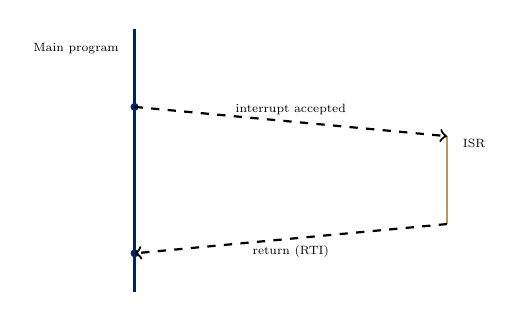
\begin{tikzpicture}[scale=0.62, transform shape,
      every node/.style={font=\small}]
    \draw[thick, primary-blue] (0,3.2) -- (0,-2.2);
    \node[font=\scriptsize, anchor=east] at (-0.2,2.8) {Main program};
    \draw[thick, primary-gold] (6.4,1.0) -- (6.4,-0.8);
    \node[font=\scriptsize, anchor=west] at (6.6,0.85) {ISR};
    \filldraw[primary-blue] (0,1.6) circle (2pt);
    \filldraw[primary-blue] (0,-1.4) circle (2pt);
    \draw[dashed, thick, ->] (0,1.6) -- (6.4,1.0)
          node[midway, above] {\scriptsize interrupt accepted};
    \draw[dashed, thick, ->] (6.4,-0.8) -- (0,-1.4)
          node[midway, below] {\scriptsize return (RTI)};
  \end{tikzpicture}
  \caption{Interrupt as a transfer of control: main program suspended at the interrupt point, control jumps to the ISR, and \texttt{RTI} returns exactly where it left off.}
  \label{fig:interrupt-transfer}
\end{figure}

\textbf{Enabling and disabling --- two independent switches.} A request reaches the CPU only when \emph{both} agree: the per-device enable bit in that device's control register (\texttt{KIRQ} for the keyboard, \texttt{DIRQ} for the display) \emph{and} the single global \texttt{IE} bit inside the processor status register (\texttt{PS}). \texttt{IE}$=0$ masks every request regardless of source --- the global panic button; the per-device bits answer ``is \emph{this} device even allowed to ask?''.

\textbf{The five-step handling scenario} (Hamacher, 6th ed., \S3.2.1, p.~106--107), applied to the keyboard with \texttt{KIRQ}$=1$, \texttt{PS.IE}$=1$:
\begin{enumerate}
  \item The keyboard sets \texttt{KIN}$=1$ and raises an interrupt-request line.
  \item The CPU finishes its \emph{current instruction} (never mid-instruction), then checks \texttt{PS.IE}.
  \item Enabled: CPU saves \texttt{PC} (and registers the ISR will clobber) into shadow registers, clears \texttt{PS.IE}$\gets0$, loads \texttt{PC} with the ISR's starting address.
  \item The ISR services the device (\texttt{MoveByte KBD\_DATA, R}, which also clears \texttt{KIN}), then executes \texttt{RTI}.
  \item \texttt{RTI} restores \texttt{PC} and sets \texttt{PS.IE}$\gets1$; the interrupted program resumes with no memory of being interrupted.
\end{enumerate}

\begin{example}[The five steps drawn on the board]
\label{ex:interruptboard}
\textbf{Board:} redraw the transfer-of-control figure as a vertical timeline and \emph{annotate each step beside the timeline as you narrate it} --- build order: (1) the two vertical timelines (main program left, ISR right); (2) the two dashed arrows labelled \texttt{interrupt accepted} and \texttt{return (RTI)}; (3) a ``step 1--5'' column down the left edge, filled in as you tell the story. \textbf{Live question before step 2:} ``the keystroke arrives while the CPU is half-way through an instruction --- can it jump now?'' (No --- it must finish the current instruction; that is why step 2 says \emph{finishes its current instruction}.)
\end{example}

\textbf{Handling multiple devices.} One request line says \emph{that} something needs attention, not \emph{which}. Two designs: \textbf{polling the sources} (the ISR checks each device's status flag in a fixed order; simple, but dispatch time grows with device count) and \textbf{vectored interrupts} (each device supplies an identifying code; hardware indexes an \textbf{interrupt-vector table} --- a table of ISR starting addresses, one entry per device --- and jumps straight there; constant-time dispatch for a little extra hardware).

\begin{example}[Two devices request simultaneously --- a ``draw the next state'' hook]
\label{ex:nestingboard}
\textbf{Board:} draw the register-level mechanism (Device~1 IRQ and Device~2 IRQ feeding \texttt{IPENDING}, \texttt{IENABLE} masking, both converging on the priority $+$ vector-table lookup that outputs the ISR start address to \texttt{PC}). Then pose the hook question: ``Device 1 (higher priority) and Device 2 both request on the same cycle; Device 1's ISR is still running when Device 2's request would normally be granted --- what happens to Device 2's request?'' Let a student answer before you reveal: if nesting is enabled and Device 2 outranks Device 1's current ISR priority, the identical five-step scenario applies recursively (Device 1's ISR plays the ``main program''); if nesting is disabled (or Device 2 is lower priority), the request stays \textbf{latched in \texttt{IPENDING}} --- not lost, not re-requested --- until Device 1's ISR re-enables interrupts and the encoder re-evaluates.
\end{example}

\begin{figure}[h]
  \centering
  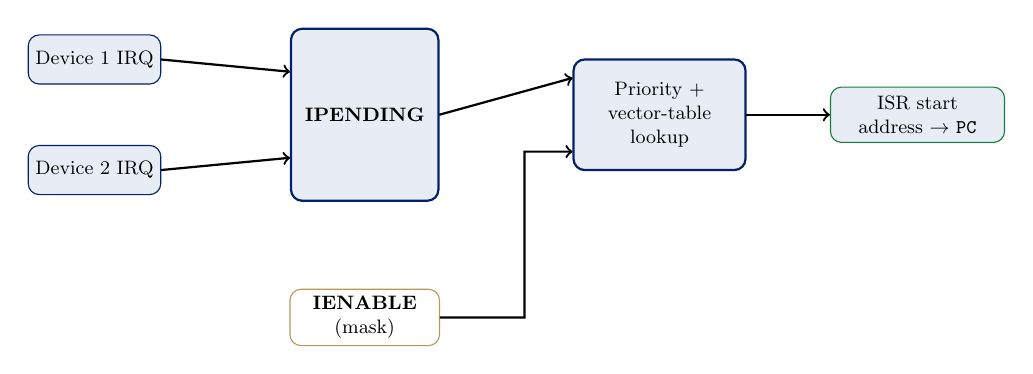
\begin{tikzpicture}[scale=0.78, transform shape,
      every node/.style={font=\small}]
    \node[draw=primary-blue, fill=light-bg, rounded corners,
          minimum width=2.0cm, minimum height=0.8cm, align=center]
          (D1) at (0,2.6) {Device 1 IRQ};
    \node[draw=primary-blue, fill=light-bg, rounded corners,
          minimum width=2.0cm, minimum height=0.8cm, align=center]
          (D2) at (0,0.8) {Device 2 IRQ};
    \node[draw=primary-blue, thick, fill=light-bg, rounded corners,
          minimum width=2.4cm, minimum height=2.8cm, align=center]
          (IPEND) at (4.4,1.7) {\textbf{IPENDING}};
    \node[draw=primary-gold, fill=white, rounded corners, text width=2.2cm,
          minimum height=0.9cm, align=center]
          (IENABLE) at (4.4,-1.6) {\textbf{IENABLE} (mask)};
    \node[draw=primary-blue, thick, fill=light-bg, rounded corners,
          minimum width=2.8cm, minimum height=1.8cm, align=center]
          (PRI) at (9.2,1.7) {Priority $+$\\vector-table\\lookup};
    \node[draw=positive, fill=light-bg, rounded corners, text width=2.6cm,
          minimum height=0.9cm, align=center]
          (OUT) at (13.4,1.7) {ISR start address $\to$ \texttt{PC}};
    \draw[->, thick] (D1.east) -- (IPEND.west |- 0,2.4);
    \draw[->, thick] (D2.east) -- (IPEND.west |- 0,1.0);
    \draw[->, thick] (IPEND.east) -- (PRI.west |- 0,2.3);
    \draw[->, thick] (IENABLE.east) -- (7.0,-1.6) -- (7.0,1.1) -- (PRI.west |- 0,1.1);
    \draw[->, thick] (PRI.east) -- (OUT.west);
  \end{tikzpicture}
  \caption{Interrupt dispatch with priority: device IRQ lines set bits in \texttt{IPENDING}; \texttt{IENABLE} masks which pending requests the priority encoder considers; the encoder plus vector-table lookup produces the winning ISR's starting address.}
  \label{fig:nesting}
\end{figure}

\begin{teachingaside}
The single most valuable sentence of this Act: \emph{polling and interrupts are the same problem with the initiative reversed} --- they move the waiting cost from CPU cycles to the hardware that detects readiness. Students who hear that once can answer the trade-off table from first principles instead of memorizing it. Also flag explicitly that interrupts do not eliminate the waiting; they relocate it.
\end{teachingaside}

\section{Topic 3: Synchronous and Asynchronous Buses}

Drop one level, from ``when does the CPU check / get notified'' to ``what do the wires actually do.'' Every interface hangs off a single shared \textbf{bus} (address, data, control lines everyone listens to). A \textbf{bus protocol} defines how a \textbf{master} (the device driving the transfer, usually the CPU) and a \textbf{slave} (the responder) coordinate one transfer without colliding. The question: when a master says ``take this data,'' how does the slave say ``not ready yet'' or ``here it is''? Two answers: \textbf{synchronous} and \textbf{asynchronous}.

\textbf{Synchronous bus:} all devices share a common \textbf{bus clock}; the master places address/data at a fixed clock edge; every slave samples at the \emph{same} edge with no per-transfer negotiation. A slow slave stretches the transfer by holding \texttt{Slave-ready} low for extra clock cycles (wait states); the master simply waits, still synchronized.

\begin{figure}[h]
  \centering
  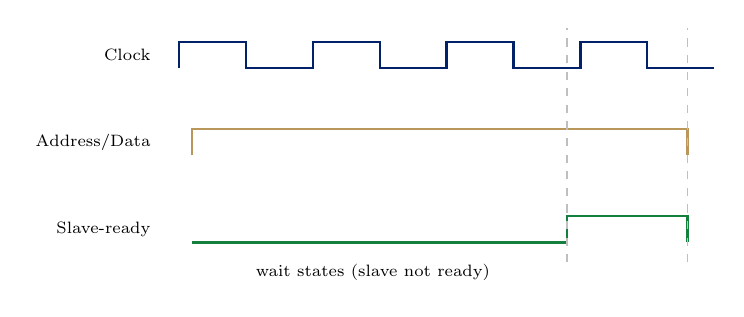
\begin{tikzpicture}[scale=0.85, transform shape,
      every node/.style={font=\scriptsize}]
    \node[anchor=east] at (-0.3,2.6) {Clock};
    \draw[thick, primary-blue]
      (0,2.4) -- (0,2.8) -- (1,2.8) -- (1,2.4) -- (2,2.4) -- (2,2.8) --
      (3,2.8) -- (3,2.4) -- (4,2.4) -- (4,2.8) -- (5,2.8) -- (5,2.4) --
      (6,2.4) -- (6,2.8) -- (7,2.8) -- (7,2.4) -- (8,2.4);
    \node[anchor=east] at (-0.3,1.3) {Address/Data};
    \draw[thick, primary-gold]
      (0.2,1.1) -- (0.2,1.5) -- (7.6,1.5) -- (7.6,1.1);
    \node[anchor=east] at (-0.3,0) {Slave-ready};
    \draw[thick, positive]
      (0.2,-0.2) -- (5.8,-0.2) -- (5.8,0.2) -- (7.6,0.2) -- (7.6,-0.2);
    \node[font=\scriptsize] at (2.9,-0.65) {wait states (slave not ready)};
    \draw[dashed, gray!50] (5.8,-0.5) -- (5.8,3.0);
    \draw[dashed, gray!50] (7.6,-0.5) -- (7.6,3.0);
  \end{tikzpicture}
  \caption{Synchronous-bus timing with wait states: address/data held valid across the transfer while \texttt{Slave-ready} stays low for several clock periods until the slow slave is ready.}
  \label{fig:sync-bus}
\end{figure}

\textbf{Asynchronous bus (full handshake):} no shared clock; master and slave exchange explicit \texttt{Master-ready}/\texttt{Slave-ready} signals, each changing only \emph{in response to} the other. Four interlocked steps: (1) \texttt{Master-ready} asserted; (2) \texttt{Slave-ready} (data valid); (3) \texttt{Master-ready} withdrawn (latched); (4) \texttt{Slave-ready} withdrawn. Each step waits for the previous one, so \textbf{bus skew} (wires arriving at slightly different times) never causes a false sample --- but every transfer pays two full round trips.

\begin{figure}[h]
  \centering
  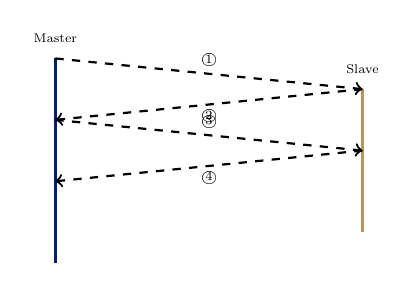
\begin{tikzpicture}[scale=0.65, transform shape,
      every node/.style={font=\small}]
    \node[font=\scriptsize] at (0,4.0) {Master};
    \node[font=\scriptsize] at (6.0,3.4) {Slave};
    \draw[thick, primary-blue] (0,3.6) -- (0,-0.4);
    \draw[thick, primary-gold] (6.0,3.0) -- (6.0,0.2);
    \draw[dashed, thick, ->] (0,3.6) -- (6.0,3.0)
          node[midway, above] {\scriptsize \textcircled{\scriptsize 1}};
    \draw[dashed, thick, ->] (6.0,3.0) -- (0,2.4)
          node[midway, below] {\scriptsize \textcircled{\scriptsize 2}};
    \draw[dashed, thick, ->] (0,2.4) -- (6.0,1.8)
          node[midway, above] {\scriptsize \textcircled{\scriptsize 3}};
    \draw[dashed, thick, ->] (6.0,1.8) -- (0,1.2)
          node[midway, below] {\scriptsize \textcircled{\scriptsize 4}};
  \end{tikzpicture}
  \caption{The asynchronous full handshake as a four-step interlocked exchange; each arrow fires only after the previous one has been observed.}
  \label{fig:async-bus}
\end{figure}

\begin{example}[Drawing both timing diagrams --- two board exercises]
\label{ex:busboard}
\textbf{Board (synchronous):} draw the clock row first (a square wave), then the address/data band held valid, then \texttt{Slave-ready} as a step rising late. Narrate the two dashed edges: the first dashed line is where \texttt{Slave-ready} finally rises; the second is where the master samples. \textbf{Live question:} ``a fast device needs zero wait states --- where would \texttt{Slave-ready} sit on this diagram?'' (Already high at the very first edge.)

\textbf{Board (asynchronous):} draw the master column and slave column first, then add the four diagonal arrows \emph{one at a time}, narrating each step's trigger: ``step 3 only fires because the master \emph{saw} step 2.'' \textbf{Prediction trap:} ``why does this never sample corrupted data?'' Let a student state ``because each side waits until it actually observes the other side's signal'' before you add the skew label.
\end{example}

\begin{example}[Wait-state arithmetic --- second instance]
\label{ex:waitstates}
\textbf{Board:} the lecture's trade-off table says synchronous is cheap per transfer but pays wait states for slow devices. Quantify it: a synchronous transfer needs 3 wait-state cycles at a 250~MHz bus clock ($1/(250\times10^6)=4$~ns per cycle) before \texttt{Slave-ready} rises, then one more period to sample: total $(3+1)\times4=16$~ns. A second instance: 5 wait states at 500~MHz ($2$~ns/cycle) $\Rightarrow$ $(5+1)\times2=12$~ns. Do the arithmetic on the board \emph{before} showing the asynchronous handshake, so the ``two round trips'' cost lands as a concrete comparison.
\end{example}

\begin{teachingaside}
Students reliably conclude ``asynchronous is strictly better'' because it tolerates skew and any speed. The counter is the per-transfer overhead: every asynchronous transfer pays two full round trips, which a fast, similar-speed synchronous bus never pays. That is precisely why high-speed processor buses are synchronous. Have the class \emph{argue} the ``why not always async?'' Socratic question from the deck --- it forces the trade-off table into a sentence.
\end{teachingaside}

\section{Topic 4: DMA and I/O Processors}

Interrupts removed the CPU's \emph{waiting}, but not its involvement in \emph{moving} the data. A disk block transfer is one word at a time; with interrupt-driven I/O the ISR executes on every word (read status, read/write data, update pointer, decrement counter, return). A 4096-byte block at 4 bytes/word is $4096/4=1024$ ISR invocations for a single block. The next step removes the CPU from the data path.

\textbf{Bus arbitration --- a third role for a device.} DMA needs a capability not yet introduced: a device other than the CPU becoming bus master. \textbf{Bus arbitration} decides which of several candidate masters gets the bus each cycle. Each candidate asserts a bus-request line (\texttt{BR}); the arbiter grants the bus to exactly one requester, by priority, over a bus-grant line (\texttt{BG}).

\begin{figure}[h]
  \centering
  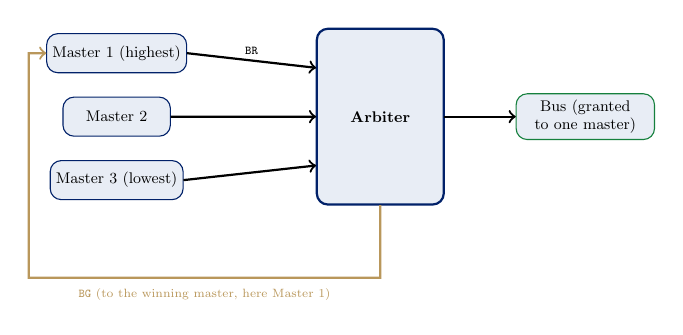
\begin{tikzpicture}[scale=0.62, transform shape,
      every node/.style={font=\small}]
    \node[draw=primary-blue, fill=light-bg, rounded corners,
          minimum width=2.2cm, minimum height=0.8cm, align=center]
          (M1) at (0,2.6) {Master 1 (highest)};
    \node[draw=primary-blue, fill=light-bg, rounded corners,
          minimum width=2.2cm, minimum height=0.8cm, align=center]
          (M2) at (0,1.3) {Master 2};
    \node[draw=primary-blue, fill=light-bg, rounded corners,
          minimum width=2.2cm, minimum height=0.8cm, align=center]
          (M3) at (0,0) {Master 3 (lowest)};
    \node[draw=primary-blue, thick, fill=light-bg, rounded corners,
          minimum width=2.6cm, minimum height=3.6cm, align=center]
          (ARB) at (5.4,1.3) {\textbf{Arbiter}};
    \node[draw=positive, fill=light-bg, rounded corners, text width=2.6cm,
          minimum height=0.9cm, align=center]
          (BUS) at (9.6,1.3) {Bus (granted to one master)};
    \draw[->, thick] (M1.east) -- (ARB.west |- 0,2.3)
          node[midway, above] {\scriptsize \texttt{BR}};
    \draw[->, thick] (M2.east) -- (ARB.west |- 0,1.3);
    \draw[->, thick] (M3.east) -- (ARB.west |- 0,0.3);
    \draw[->, thick, primary-gold] (ARB.south) -- (5.4,-2.0) -- (-1.8,-2.0) -- (-1.8,2.6) -- (M1.west);
    \node[font=\scriptsize, primary-gold] at (1.8,-2.35)
          {\texttt{BG} (to the winning master, here Master 1)};
    \draw[->, thick] (ARB.east) -- (BUS.west);
  \end{tikzpicture}
  \caption{Bus arbitration: three candidate masters assert \texttt{BR}; the arbiter grants \texttt{BG} to exactly one requester, by priority, at a time.}
  \label{fig:arbitration}
\end{figure}

\begin{example}[Arbitration order --- two instances]
\label{ex:arbboard}
\textbf{Board:} draw the three masters, the arbiter box, and the \texttt{BR} lines first, then the \texttt{BG} return path, then label the priority order. Narrate the lecture's instance (all three request the same cycle $\Rightarrow$ grant Master 1; on release, re-evaluate the still-pending requests and grant Master 2 next, then Master 3). \textbf{Live question:} ``add a Master 4 with \emph{lowest} priority, all four requesting on the same cycle, each releasing promptly --- what is the service order?'' (Strict priority: 1, 2, 3, 4 --- the queue is served purely by priority because all were pending from the start and no new requests reorder it.)
\end{example}

\textbf{From arbitration to DMA.} Once a device can become bus master, it can transfer data \emph{directly to/from memory}, with no CPU instruction touching the data; the CPU is interrupted once, when the whole block finishes. \textbf{Honest-phrasing note:} this 6th edition of Hamacher describes exactly this mechanism in \S7.3 but never names it ``DMA''; the term and standard treatment follow Stallings Ch.~7 (chapter-level, not page-indexed).

\textbf{DMA (general/standard treatment --- Stallings Ch.~7).} A \textbf{DMA controller} is given a source/destination address and a word count by the CPU, becomes bus master (via arbitration), and transfers the whole block directly to/from memory, interrupting the CPU only when the \emph{block} completes. Pro: CPU involvement drops from one ISR per word (1024 for the running 4096-byte block) to one setup $+$ one completion interrupt --- constant in block size. Con: the DMA controller and CPU now compete for the same memory bus (\textbf{cycle stealing}); extra hardware required.

\textbf{IOP (general/standard treatment --- Stallings Ch.~7).} An \textbf{I/O processor} generalizes DMA one step further: a dedicated processor given a whole \emph{channel program} (several transfers, formats, simple decisions) executes it independently, interrupting the main CPU only when the entire program completes. DMA offloads \emph{moving}; an IOP offloads \emph{managing a sequence} --- the difference is how much decision-making is delegated away from the CPU.

\begin{example}[ISR count vs.\ DMA cost --- second instance]
\label{ex:dmaboard}
\textbf{Board:} recompute the lecture's 4096-byte example for an 8192-byte block (4 bytes/word): interrupt-driven needs $8192/4=2048$ ISR invocations; DMA still needs exactly 2 CPU events (1 setup $+$ 1 completion interrupt). \textbf{Prediction trap before revealing:} ``guess how many ISR invocations an 8192-byte block needs, given the 4096-byte case needed 1024.'' (Exactly double --- 2048, linear in block size --- while DMA's 2 is unchanged, which is the entire argument for DMA.) Draw the cycle-stealing sketch while narrating: the DMA controller and CPU both want the same memory bus; a stolen cycle is a CPU memory access that has to wait.
\end{example}

\begin{teachingaside}
Two misconceptions recur. (1) ``DMA halts the CPU.'' No --- it steals \emph{bus cycles}, so the CPU is delayed only when it wants the memory bus, and only for one cycle at a time, not halted wholesale. (2) ``Polling vs.\ interrupt is a ranking of quality.'' It is a \emph{latency-vs-overhead} trade-off that depends on the device's rate and how much else the CPU has to do. The closing head-to-head table (CPU cost per word and per block for Polling/Interrupts/DMA/IOP) is the artifact students should be able to reconstruct, not memorize --- every cell follows from ``who is on the critical path.''
\end{teachingaside}

\section{Summary}

\textbf{The one-sentence spine:} every I/O technique moves the cost of ``someone must notice the device is ready, and someone must move the data'' somewhere else --- CPU cycles (polling), interrupt-handling hardware (interrupts), per-transfer wire delay (asynchronous buses), or dedicated data-path hardware (DMA/IOP) --- and none of them is free.

\begin{itemize}
  \item \textbf{Memory-mapped I/O} places device registers in the normal address space; \textbf{polling} tests a status flag (\texttt{KIN}/\texttt{DOUT}) in a loop and wastes CPU time in proportion to the device/CPU speed gap.
  \item \textbf{Interrupts} reverse the initiative: \texttt{PS.IE} and per-device enables (\texttt{KIRQ}/\texttt{DIRQ}) gate delivery; \textbf{vectored interrupts} dispatch in constant time via \texttt{IPENDING}/\texttt{IENABLE} and the interrupt-vector table; nesting lets a higher-priority request interrupt an ISR recursively, otherwise requests stay latched in \texttt{IPENDING}.
  \item \textbf{Synchronous buses} trust a shared clock (cheap per transfer, wait states for slow slaves); \textbf{asynchronous buses} trust nothing (a \texttt{Master-ready}/\texttt{Slave-ready} full handshake --- skew-immune, but two round trips per transfer).
  \item \textbf{Arbitration} (\texttt{BR}/\texttt{BG}) lets a device become bus master --- the basis for \textbf{DMA} (block transfer, one completion interrupt, cycle stealing) and \textbf{IOP} (whole channel programs; general treatment per Stallings Ch.~7).
\end{itemize}

\textbf{Bridge to Week 9:} Weeks 1--8 built a CPU that computes, controls itself, and now moves data to and from slow devices. Week 9 asks the same speed-mismatch question about \emph{memory itself} (DRAM is far slower than the CPU): cache memory, mapping functions, and replacement policies.

\end{document}
